%!TEX root = depicto-top.tex
%%%%%%%%%%%%%%%%%%%%%%%%%%%%%%%%%%%%%%%%%%%%%%%%%%%%%%%%%%%%%%%%%%%%%%%%%%%%%%
%% The Pipeline
%%%%%%%%%%%%%%%%%%%%%%%%%%%%%%%%%%%%%%%%%%%%%%%%%%%%%%%%%%%%%%%%%%%%%%%%%%%%%%
% \documentclass{standalone}
% \begin{document}
%-----------------------------------------------------------------------------

%%%%%%%%%%%%%%%%%%%%%%%%%%%%%%%%%%%%%%%%%%%%%%%%%%%%%%%%%%%%%%%%%%%%%%%%%%%%%%
%% PART I
%%%%%%%%%%%%%%%%%%%%%%%%%%%%%%%%%%%%%%%%%%%%%%%%%%%%%%%%%%%%%%%%%%%%%%%%%%%%%%

% \chapter{The \depicto\ pipeline (I): Parsing the picto-input }
% \chapter{\depicto\ (I): Deep parsing the pictographic input}
\chapter{\depicto\ I: Deep parsing \sclera}
\label{chap:pipeline1}

This is the first of two chapters that introduce the \depicto\ pipeline by
looking at each of its consecutive grammar modules. The focus here is the
module responsible for parsing a string of \sclera\ symbols and extracting as
much semantic information from it as possible. First,
\cref{sec:picto-identifiers} shows how \sclera\ symbols are passed to the
parser as strings of identifiers. Next, \cref{sec:mini-sclera} details the
initial stage of designing a grammar that can be used to process such strings.
A (hypothetical) grammar of \sclera\ is sketched out, the LinGO
Grammar Matrix customization system is used to quickly obtain a working grammar
prototype, and an initial set of modifications is made so as to re-introduce
missing relations of quantification. As a brief intermezzo,
\cref{sec:sclera:mrsoutput} gives a walkthrough of the \mrs\ output yielded by
the \sclera\ analysis module. Finally, \cref{sec:casestudies} describes three
case studies which demonstrate how the initial model of \sclera\ can be
extended with a view to (a) increasing its semantic accuracy and (b)
incorporating complex, or `compound', pictographs. Note that, all in all, this
chapter concerns the most innovative contribution of this thesis. As a result,
in contrast with the chapter that comes after, it may at times be observed that
brevity is foregone in favor of extra clarity.

% \section{A simple example} % skipped, for now
% Because it's always nice to have something concrete.

%-----------------------------------------------------------------------------

\section{Parser input: A note on picto identifiers}
\label{sec:picto-identifiers}

The \depicto\ pipeline analyses sequences of selected pictographs not as actual
images, but as strings of identifiers with which individual pictographs are
associated. These identifier \emph{tokens} are matched against lexical entries
defined on the parsing grammar's lexicon. (Unlike natural language tokens,
pictograph identifiers are not subject to inflectional rules, spelling mistakes
or other sources of variation, so matching is non-partial.) In Matrix-based
grammars, the specific part of the lexical entry against which identifiers are
matched is a string value specified on the feature
\textsc{stem}\footnote{Non-Matrix grammars use a functionally identical
feature, but use different names for it. For instance, the English Resource
Grammar \citep{flickinger2014towards} uses \textsc{phon}, which is in
accordance with \citep{pollard1994head} as well as the off-shoot \textsc{hpsg}
`variant' \textsc{sbcg} \citep{boas2012sign}}. To illustrate this,
\cref{ex:exampleSTEM} shows the \tdl\ description of a typical lexical entry,
of which the AVM equivalent is given directly below, in
\cref{ex:exampleStemAVM}.

\begin{exe}\ex\label{ex:exampleSTEM}
    \begin{verbatim}
dog := common-noun-lex &
  [ STEM < "dog" >,
    SYNSEM.LKEYS.KEYREL.PRED "_dog_n_rel" ].
    \end{verbatim}
\end{exe}

\begin{exe}\ex\label{ex:exampleStemAVM}
    \begin{avm}
        < \textnormal{dog},
                 [ \asort{common-noun-lex}
                   stem \; \< \avmstring{dog} \> \\
                   synsem|lkeys|keyrel|pred &
                       \avmstring{\_dog\_n\_rel} ] >
    \end{avm}
\end{exe}

Pictograph identifiers are passed to the parser as simple character strings
(i.e., no complex data structures are involved), separated by any number of
horizontal white spaces.

The naming convention to which these pictograph identifiers adhere warrants
slightly more detailed discussion, not least because there are, in fact,
several naming systems to choose from.

The first, and easiest, option (at least, initially) involves identifying
pictographs with the names of the files in which they are individually stored.
These filenames, whose extension is stripped away, either convey some part of
the pictograph's sense or describe the appearance of the pictograph itself. An
example of a hypothetical lexical entry where the identifier value of
\textsc{stem} is thus formatted is given in \cref{ex:filenameID}.

\begin{exe}\ex\label{ex:filenameID}
    \small
    \begin{verbatim}
thunderstorm := common-noun-lex &
  [ STEM < "thunder", "and", "lightning" >, ; from: "thunder and lightning.png"
    SYNSEM.LKEYS.KEYREL.PRED "_thunderstorm_n_rel" ].
    \end{verbatim}
\end{exe}

Ignoring the fact that not all filenames correspond to the image's meaning,
this naming strategy has two major drawbacks In the first place, it restricts
the parser's grammar model entirely to the \sclera\ symbol set, whereas the aim
of \depicto\ is to be applicable to at least a subset of other symbol sets,
too. In the second place, filename-based identifiers make it, if not
impossible, needlessly complicated to generalize over pictographs that are
synonymous as far as the system is concerned: multiple lexical entries bearing
the same semantic meaning could be provided for each picto `synonym', but this
would be a costly procedure inevitably requiring manual intervention, since
synonymy is not always suggested by the filename alone.

A different approach to naming pictograph identifiers piggy-backs on work by
\citet{vandeghinste2014linking} on linking pictographs to the English WordNet
database \citep{miller1995wordnet} and international variants thereof, such as
the Cornetto database for Dutch (discussed in \cref{sub:picto2text};
\citep{vossen2007cornetto}). Just as in the Text2Picto and Picto2Text systems
(again, see \cref{sub:picto2text}), pictographs are identified with the ID tag
of a linked \emph{synonym set}, as the value of \textsc{stem} in
\cref{ex:synsetID} shows. Synset IDs vary across different WordNet databases,
but they are easily made compatible with the right database query. Moreover,
the pictograph--WordNet dictionaries developed by
\citet{vandeghinste2014linking} are additionally linked to the \emph{Beta}
symbol set (discussed in \cref{sub:Beta}), so that a grammar model of \sclera\
in which pictographs are identified by linked synset IDs has the potential, in
theory, to be applied to \emph{Beta} as well.

\begin{exe}\ex\label{ex:synsetID}
    \small
    \begin{verbatim}
door := common-noun-lex &
  [ STEM < "d_n-27669" >,
    SYNSEM.LKEYS.KEYREL.PRED "_door_n_rel" ].
    \end{verbatim}
\end{exe}

Still in an early stage of prototyping, the \depicto\ system does not make use
of synset IDs, yet. This has to do, in part, with the fact that non-content
words are omitted from WordNet. As the inventory in \cref{sub:scleraInventory}
suggests, this does not present such a big problem for \sclera, with its
general lack of prepositions, determiners, auxiliaries, etc., although personal
pronouns do exist in \sclera, as well as a small group of operators (conveying,
e.g., conjunction, negation, lack of permission). For these, an additional set
of identifiers must be devised. Granted, this does not present too much of a
hurdle. More relevant to the motivation for not using synset IDs in the current
version of \depicto, yet similarly practical in nature, is a problem that comes
up in the early stages of grammar development, when testing a grammar is most
easily done \emph{not} by some automatic process, but by manually typing out
test strings that include the phenomenon being tested for. Synset IDs, as
\cref{ex:synsetID} might suggest, are not particularly easy to remember and,
much like an overly complicated password, comprise enough unpredictable
characters to be prone to typographic error. The result is that manual methods
of grammar testing quickly become tiresome.

To aid the process of prototyping, therefore, pictographs are currently passed
to the analysis module as simple English lemmas, as shown in \cref{ex:lemmaID}
and \cref{ex:lemmaID2}. (In the case of complex pictographs, the constituent
semantic parts are additionally separated by \emph{underscores}.) This approach
represents a comfortable compromise between the comparative readability of
filename-based identifiers and the (currently unexplored) potential of being
linked to the WordNet database that comes with synset IDs (from which the
current approach gets its lemmas). This compromise is only temporary, however.
Although the lexicon of the grammar model is small enough not to cause any
problems at the moment, further growth will necessitate a transition to a
synset ID-based naming approach.

\begin{exe}\ex\label{ex:lemmaID}
    \small
    \begin{verbatim}
dog := common-noun-lex &
  [ STEM < "dog" >,
    SYNSEM.LKEYS.KEYREL.PRED "_dog_n_rel" ].
    \end{verbatim}
\end{exe}

\begin{exe}\ex\label{ex:lemmaID2}
    \small
    \begin{verbatim}
walk_v := common-verb-lex &
  [ STEM < "walk" >,
    SYNSEM.LKEYS.KEYREL.PRED "_walk_v_rel" ].
    \end{verbatim}
\end{exe}

\section{A first crack at a grammar of \sclera}
\label{sec:mini-sclera}

This section details the construction of a constraint-based grammar model that
can be used to `deep' parse strings of \sclera\ symbol identifiers. Drawing
entirely on the \delphin\ resources introduced in \cref{sec:delph-in}, this
grammar is used by the analysis module to produce semantic representations of
the \sclera\ input. Before looking at the modelling process itself, however, we
briefly examine the inherent assumption that \sclera\ \emph{can be modelled} in
the first place. The first next section presents an illustration of a number of
`typical' \sclera\ strings and shows how these can be analysed in natural
language terms. The phenomena which a simple grammar should aim to cover are
outlined here as well, with the necessary caveats here and there. With these
preliminaries in place, we see how an initial starter grammar is obtained
through the Matrix customization system (see \cref{ssub:matrixcustomization})
and how this is extended to account for the most salient structural properties
of the \sclera\ input as well as basic word order patterns. Next, we look at
one of the first major milestones in the construction of the \sclera\ grammar,
namely, the re-introduction of (non-existent) determiners onto the semantic
representations of parsed \sclera\ utterances (recall the inventory of \sclera\
provided in \cref{sub:scleraInventory}). This process of \emph{rule-based
semantic enrichment} (a notion borrowed from \citet{crysmann2012towards}), of
which two more examples are given in \cref{sec:casestudies}, goes a long way in
establishing the viability of an approach that, as we explain, aims to treat
\sclera, or indeed any pictographic language, not simply as an underspecified
analogue of some natural language, but as a language in its own right, with its
own rules and idiosyncrasies. This part of the modelling process is therefore
discussed in a separate subsection (\ref{sub:MissingDeterminers}).

\subsection{\sclera\ as a (natural) language}
\label{sub:sclerastrings}

Building on the inventory of \sclera\ given in \cref{sub:scleraInventory}, we
now look at how individual pictographs can be combined to form meaningful
sequences, or strings, much like the words of a given language can be combined
into arbitrarily complex utterances. In fact, with much of the \sclera\ set
consisting of pictographs depicting concepts that are generally the domain of
verbs and nouns, it is possible to project large parts of our knowledge of
natural language syntax onto the surface structure of \sclera\ strings, as
\cref{ex:sclera:i-walk} illustrates with a simple example.

\begin{exe}
    \ex \label{ex:sclera:i-walk}\attop{
    \gll
       {\includegraphics[width=2cm]{sclera/ik}\hspace{0.5cm}}
       {\includegraphics[width=2cm]{sclera/wandelen}}\\
       \emph{I} \emph{walk}\\
    }
    \glt `I walk.'
\end{exe}

The picto sequence in \cref{ex:sclera:i-walk} can be analysed structurally as
comprising an intransitive `verb' picto \emph{walk} and a `pronoun' picto
\emph{I}, which serves as the subject of the verb.

Note that, despite appearances, the pictographs themselves do not encode mutual
grammatical agreement. This can be seen more clearly in the example in
\cref{ex:sclera:dog-see-bus}, which shows a similar single `picto clause',
except here the `verb' picto, \emph{see}, depicts a process that is
conceptually transitive, where the `noun' picto \emph{bus} serves as object.

\begin{exe}
    \ex \label{ex:sclera:dog-see-bus}\attop{
    \gll
       {\includegraphics[width=2cm]{sclera/hond3}\hspace{0.5cm}}
       {\includegraphics[width=2cm]{sclera/zien}\hspace{0.5cm}}
       {\includegraphics[width=2cm]{sclera/bus}} \\
       \emph{dog} \emph{see} \emph{bus} \\
    }
    \glt `The dog sees the bus.'
\end{exe}

Ignoring for the time being the missing determiners in
\cref{ex:sclera:dog-see-bus}, it is, so far, possible to conclude that `verb'
pictos can be analysed in much the same way as ordinary verbs with regard to
their valency, despite the fact that, by default, they do not encode for
number, person, tense, aspect or mood, nor are their arguments marked for
number, person or gender (leaving quantification aside for now). Note, too,
that both examples are internally structured according to a
\emph{subject-verb-object} (henceforth \emph{SVO}) element order. Since
\sclera\ is virgin territory as far as its hypothetical syntax is concerned,
there is no evidence to suggest that this is the only word order that a grammar
of \sclera\ should expect, much less that it is the one which ID users would
prefer; however, in the examples that follow, as well as in the grammar model
whose design these examples ultimately inform, \emph{SVO is the word order that
is assumed}\footnote{As discussed later, in \cref{subconc:eval:main}, this is a
serious limitation of the current version of the system. Nevertheless, it is
currently maintained as the only permitted word order because it prevents
structural ambiguity (which arises quickly in the absence of inflection and
other syntactic markings) and allows the analysis of valency and word order to
be implemented relatively easily. Moreover, the combination of multiple
permitted word order patterns in a single grammar represents a complex
undertaking, although, ultimately, it is a goal of the \sclera\ grammar.}.

Structurally, `adjectival' pictographs can also be hypothesized to have
combinatory potential, as examples \cref{ex:sclera:purple-bike} and
\cref{ex:sclera:happy-dog} suggest. Here, \emph{purple} and \emph{happy} can be
seen to modify the `noun' pictos \emph{bike} and \emph{dog}, respectively. Of
course, this is not the only function that such adjectival pictographs can
fill: they can also serve as `nouns' and predicative complements, the latter
function demonstrated in \cref{ex:sclera:dog-is-happy}. (Note that, while
interesting, `adjective' pictos form a minority within the \sclera\ set.
Further, the predicative use of adjectives is not subject to modelling.)

\begin{exe}
    \ex \label{ex:sclera:purple-bike}\attop{
    \gll
       {\includegraphics[width=2cm]{"sclera/kleur paars"}\hspace{0.5cm}}
       {\includegraphics[width=2cm]{sclera/fiets}}\\
       \emph{purple} \emph{bike}\\
    }
    \glt `The purple bike.'
    %
    \ex \label{ex:sclera:happy-dog}\attop{
    \gll
       {\includegraphics[width=2cm]{"sclera/blij"}\hspace{0.5cm}}
       {\includegraphics[width=2cm]{sclera/hond1}}\\
       \emph{happy} \emph{dog}\\
    }
    \glt `The happy dog.'
    %
    \ex
    \label{ex:sclera:dog-is-happy}
    *predicative use of adjective picto \\
    \attop{
    \gll
       {\includegraphics[width=2cm]{"sclera/hond1"}\hspace{0.5cm}}
       {\includegraphics[width=2cm]{sclera/blij}}\\
       \emph{dog} \emph{happy}\\
    }
    \glt `The dog is happy.'
\end{exe}

The foregoing examples all have in common that they involve pictographs
depicting a conceptual simplex: each pictograph corresponds to a single concept
and (in English at least) to single word. However, recall from the inventory of
\sclera\ given in \cref{sub:scleraInventory} that \sclera\ additionally
comprises a large set of pictographs which depict conceptual \emph{complexes}.
These `complex' pictographs generally center on a conceptual process (verb) and
`bundle', as it were, one or more concrete arguments associated with this
process.

There are several kinds of complex pictogaphs. The least problematic for a
traditional constituent-based approach is illustrated in
\cref{ex:sclera:i-go-school}.

\begin{exe}
    \ex\label{ex:sclera:i-go-school}
    \attop{
    \gll
       {\includegraphics[width=2cm]{sclera/ik}\hspace{0.5cm}}
       {\includegraphics[width=2cm]{"sclera/school gaan 3"}\hspace{0.5cm}}\\
       \emph{I} \emph{go+school} \\
    }
    \glt `I $
        \left\{
            \begin{tabular}{@{}l@{}}
                go \\
                am going
            \end{tabular}
        \right\}
        $ to school.'
\end{exe}

The complex picto in \cref{ex:sclera:i-walk}, \emph{go+school}, depicts two
concepts: a process of `going', and the target of movement, i.e., `school'. In
English (and, incidentally, in Dutch also) the latter is expressed as an
obligatory locative complement, set off by a preposition. Syntactically,
complex pictographs of this kind can be analysed as partially `saturated'
verbal constituents that are still `seeking' an element to fill their subject
slot. Other kinds of complex pictographs, however, may combine with optional
complements, as illustrated by \emph{give+present} in example
\cref{ex:sclera:teacher-give-present}. Such complex pictographs are slightly
less evident, but are generally compatible with SVO phrase structure analyses.

\begin{exe}
    \ex \label{ex:sclera:teacher-give-present}
    \attop{
    \gll
       {\includegraphics[width=2cm]{sclera/leerkrachte}\hspace{0.5cm}}
       {\includegraphics[width=2cm]{"sclera/geschenkje geven"}\hspace{0.5cm}}
       {\includegraphics[width=2cm]{sclera/jij}} \\
       \emph{teacher} \emph{give+present} \emph{you} \\
    }
    \glt `The teacher gives a present to you.'
\end{exe}

Other pictographs depict conceptual complexes that correspond to entire
clauses, such as \emph{dog+barks} in \cref{ex:sclera:dog-barks}.

\begin{exe}
    \ex \label{ex:sclera:dog-barks}
    \attop{
    \gll
       {\includegraphics[width=2cm]{sclera/hond-blaffen}\hspace{0.5cm}}\\
       \emph{dog+barks}\\
    }
    \glt `The dog barks.'
\end{exe}

Like the absence of determiners/quantifiers, complex pictographs are a feature
of \sclera\ that sets it apart from most `true' natural languages.
Unsurprisingly, therefore, including these pictographs in a grammar model of
\sclera\ requires some slightly different machinery, particularly to make
`constituent' concepts accessible to other parts of the grammar, so that
sequences like in \cref{ex:sclera:happy-dog-barks} are grammatical. We return
to the integration of complex pictographs in \cref{subs:cs:complex-pictos}.
Easier to analyse, simplex pictographs will form the basis of the initial
grammar.

\begin{exe}
    \ex \label{ex:sclera:happy-dog-barks}
    \attop{
    \gll
       {\includegraphics[width=2cm]{sclera/blij}\hspace{0.5cm}}
       {\includegraphics[width=2cm]{sclera/hond-blaffen}\hspace{0.5cm}}\\
       \emph{happy} \emph{dog+barks}\\
    }
    \glt `The happy dog barks.'
\end{exe}

To the best of my knowledge, there currently exist no `corpora' of pictographic
text. The reasons for this are not hard to intuit. Popular and accessible
pictograph-to-text systems are few and far between (hence, the contribution of
this thesis!). If data about how these systems are used collected, it is not
shared. Yet even if it were, pictographic symbol sets vary, making comparison
difficult. As a result of all this, modelling \sclera\ is less a descriptive
than a creative process. Indeed, all the example strings presented in this
sketch are hypothetical, albeit based on linguistic knowledge. As a preface to
the next section, the assumptions which guide this `armchair' approach, as well
as the aims of the forthcoming grammar model, are summarised below.

\paragraph{Grammar aims}

\begin{itemize}
    \item Coverage of simplex picto `(pro)nouns', `verbs', and `adjectives', bearing in mind their underspecified status.
    \item Theory of picto valency/subcategorization patterns
    \item Analysis of missing determiners (\cref{sub:MissingDeterminers}).
    \item Integration of complex pictos.
    \item Ability to parse simple main/matrix clauses and noun phrases
\end{itemize}

\paragraph{Assumptions}

\begin{itemize}
    \item \sclera\ \emph{has} a grammar that can be modelled
    \item The input to the \sclera\ parser consists of lemmas that are
          morpholgically atomic.
    \item The elements on the \sclera\ input adhere to subject-verb-object
          order.
    \item The input can be resolved to a complete main clause or to a
          noun phrase.
\end{itemize}

\subsection{Setting up with the LinGO Matrix}
\label{subs:settingup:lingo}

The starting point for the construction of an implemented grammar of \sclera\
is the \lingo\ Grammar Matrix customization system (introduced in
\cref{ssub:matrixcustomization}). This system, to rephrase its basic function,
generates language-specific extensions of a core type hierarchy, viz., the
\lingo\ Matrix, based on a number of (interactively provided) statements about
properties of the language being modelled.

For ease of prototyping, however, the language that is \emph{actually} modelled
in this step is not \sclera, but the other language with which this thesis
deals, i.e., Dutch (to which we return in the next chapter). This may seem
somewhat confusing at first, particularly at the current level of abstraction,
but the idea is simple and bears mentioning sooner rather than later. As the
observations in the previous section suggest, \sclera\ can (though not
necessarily) be analysed as an SVO language and, as such, shows some
amenability to the mechanisms used in analyses of such languages. Dutch is an
SVO language, too (at least, at certain levels, which I will say more about
later). Thus, one can expect some overlap between \sclera\ and Dutch,
especially on the level of their type hierarchies. Since these grammars are
developed in parallel anyway, from an engineering standpoint, it makes sense to
capitalize on such overlap so that those parts which both grammars have in
common need not be defined twice. Therefore, we opt to use the grammar
customization step to obtain a grammar of Dutch, from which the grammar of
\sclera\ inherits \emph{part} of its type hierarchy. Crudely put, the \sclera\
grammar is an underspecified variant of a model of Dutch (though English would
have worked just as well) with a few \sclera-specific additions, which are
introduced in the following sections. However, this does not mean that the
\sclera\ grammar will be indefinitely tethered to the grammar of Dutch: it is a
marriage of convenience, not necessity. Eventually, the two will be untangled
into two discrete grammars. For reference purposes,
\cref{ex:table:scleraComponents} shows how the \sclera\ grammar's components
are related with respect to the names of the associated files.

\begin{exe}
    \ex\label{ex:table:scleraComponents}\attop{
    \small
    \begin{tabular}[h]{ p{5.4cm} | p{5.9cm} }
        \hline
        \textbf{Exclusive to \sclera} & \textbf{Inherited from Dutch grammar} \\
        \hline
        \texttt{mini-sclera.tdl}\newline(\sclera-specific type hierarchy; Developed in sections \ref{sub:MissingDeterminers} and \ref{sec:casestudies}) & \texttt{matrix.tdl}\newline(\lingo\ Matrix core type hierarchy ($\pm$ 3800 lines)) \\
        \texttt{lexicon.tdl}\newline(contains lexical entries for pictograph identifiers) & \texttt{mini-dutch.tdl} \newline (type hierarchy of Dutch) \\
        \texttt{rules.tdl}\newline(contains phrase rule entries) & \texttt{head-types.tdl} \newline(recent addition to Matrix (not discussed); defines disjunctive head types) \\
        \texttt{lrules.tdl}\newline(contains lexical rule entries) & \texttt{roots.tdl}\newline(list of structures which can serve as start symbol) \\
        \texttt{config.tdl}\newline(Initial configuration file used by \ace\ during compilation; concerns settings) & \texttt{labels.tdl} \newline(specifies labels for nodes in syntax trees (forwhen using visual modes)) \\
        \texttt{mini-sclera-top.tdl}\newline(Second \ace\ configuration file; points compiler to appropriate files) & \texttt{semi.vpm}\newline(Virtual Property Mapping interface (Not introduced in \cref{ssub:delphinstructure} on account of its rather technical nature; mediates between `internal' and `external' \mrs\ representations; see the \delphin\ wiki entry at  \href{http://moin.delph-in.net/RmrsVpm}{\texttt{moin.delph-in.net/RmrsVpm}})) \\
        \hline
    \end{tabular}
    }
\end{exe}

To recapitulate, the result of the customization step is \emph{actually} an
initial grammar of Dutch, from which an initial grammar of \sclera\ is derived.
Although the two grammars bifurcate slightly as they are extended later on
(large parts of either are, in fact, later re-written or replaced with patches
from other \delphin\ grammars), at this stage, the grammar of \sclera\ can be
thought of simply as a less specific, i.e., more `permissive', variant of the
grammar of Dutch. The grammar inherits all of the other's type constraints, but
leaves these underspecified where necessary, for instance, when a given feature
is not relevant.

The primary locus of underspecification is the lexicon. To illustrate this,
compare the lexical entry for \emph{hond} (`dog') in the grammar of Dutch
\cref{ex:Dutch:hond}) to the lexical entry for the picto \emph{dog} in the
grammar of sclera \cref{ex:Sclera:dog2}. (Note that the pictograph
identifier, specified on the list value of the \textsc{stem} attribute, is provided as a simple lemma, as discussed in \cref{sec:picto-identifiers}.)

\begin{exe}
    % \label{}
    \ex\label{ex:Dutch:hond} Lexical entry for Dutch \emph{hond} (`dog')\\
    \small
    \begin{verbatim}
hond := femmasc-count-sg-noun-lex &
  [ STEM < "hond" >,
    SYNSEM.LKEYS.KEYREL.PRED "_hond_n_rel" ].
    \end{verbatim}
    \ex\label{ex:Sclera:dog2} Lexical entry for picto depicting `dog'\\
    \small
    \begin{verbatim}
dog := common-noun-lex &
  [ STEM < "dog" >,
    SYNSEM.LKEYS.KEYREL.PRED "_dog_n_rel" ].
    \end{verbatim}
\end{exe}

The types with which these lexical entries are identified, viz.,
\emph{femmasc-count-sg-noun-lex} and \emph{common-noun-lex}, are situated on
different levels of the type hierarchy. As the local hierarchy in
\cref{ex:scleragram:typeh:nouns} shows, \emph{common-noun-lex} is a supertype
of \emph{femmasc-count-sg-noun-lex}. It inherits from \emph{obl-spr-noun-lex}
itself, which in turn multiply inherits from several other general types. (The
dashed edges between tree nodes indicate where the hierarchy has been
purposefully simplified.) Lexical entries of the type \emph{common-noun-lex},
an AVM example of which is given in \cref{ex:sclera:common-noun}, have a
\textsc{head} attribute that takes values of the type \emph{noun} (which can be
specified for the feature \textsc{case}), require one \emph{obligatory}
argument\footnote{See \cref{sub:MissingDeterminers}}, which is identified with
the value of the SPecifieR (\textsc{spr}) attribute (used to build
determiner/quantifier-noun phrases), and, on a semantic level, have additional
appropriate features \emph{person}, \emph{number}, and \emph{gender}, which
correspond to \mrs\ variables, but \emph{common-noun-lex} does not stipulate
any constraints on the values of these \mrs\ variables. As a result, the
lexical entry for the pictograph `dog' is appropriately identified with the
part-of-speech category `noun', but is left entirely underspecified with
respect to the features number, person and (since this varies from language to
language) gender. By contrast, the types used in the lexicon of the grammar of
Dutch are more specific. For instance, by inheriting from
\emph{femmasc-count-sg-noun-lex}, the lexical entry in \cref{ex:Dutch:hond} is
defined explicitly as being singular, non-neuter (feminine or masculine), and
count (requiring an explicit determiner). This is appropriate because these
features are relevant to the syntax of Dutch.

\begin{exe}
    \ex\label{ex:sclera:common-noun}
    \vspace{0.5cm}
    \begin{avm}
        [ \asort{common-noun-lex}
          stem \; < \avmstring{dog} > \\
          synsem|local & [ cat & [ head \; [ \asort{noun}
                                             case & case \\
                                             mod & \<\;\> ] \\
                                 val [subj & \<\;\> \\
                                      spr & \< @1
                                        [ local|cat|head & det \\
                                          opt \; \textnormal{-}  ] \> \\
                                          comps & \<\;\> ] ] \\
                           cont & [ hook|index|png\;[ \asort{ref-ind}
                                                      per & person \\
                                                      num & number \\
                                                      gend & gender ] \\
                                  rels \; < [
                                         \asort{ep}
                                          pred & \avmstring{\_dog\_n\_rel} ] >\\
                                   hcons \; \<\;\> ]  ] \\
          arg-st \; \< @1 \>  ]
    \end{avm}
\end{exe}

\begin{exe}
    \ex\label{ex:scleragram:typeh:nouns}\attop{
    \tikzset{every tree node/.style={anchor=base}}
    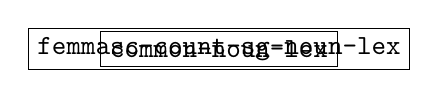
\begin{tikzpicture}
        \Tree  [.\texttt{lex-item} \edge[dashed];
               [.\texttt{basic-noun-lex} \edge[dashed];
               [.\texttt{noun-lex} \edge[dashed];
               [.\texttt{obl-spr-noun-lex}
               [. \node[draw] {\texttt{common-noun-lex}};
               \edge[thick];
               [. \node[draw] {\texttt{femmasc-count-sg-noun-lex}}; ]
               \edge[dashed];
               [.\texttt{femmasc-count-pl-noun-lex} ] ] ] ] ] ]
                % ]
    \end{tikzpicture}
    } % attop
\end{exe}

`Verb' pictographs in the lexicon of the \sclera\ grammar are similarly
identified with comparatively general lexical types. As may be intuited
partially from the associated type names, the constraints for which entries in
the Dutch grammar are specified (including \emph{person}, \emph{number}, and
\emph{tense}) are left underspecified in equivalent entries in the grammar of
\sclera. Once again, an illustration of the (local) type hierarchy, given in
\cref{ex:scleragram:typeh:intrans}, does much in the way of clarity.

\begin{exe}
    % \label{}
    \ex\label{ex:dutch:slaapt}
        \small
        \begin{verbatim}
slaapt := intrans-2nd-or-3rd-sg-verb-lex &
  [ STEM < "slaapt" >,
    SYNSEM.LKEYS.KEYREL.PRED "_slapen_v_rel" ].
        \end{verbatim}
    \ex\label{ex:sclera:sleep}
    \small
    \begin{verbatim}
sleep := intrans-verb-lex &
  [ STEM < "sleep" >,
    SYNSEM.LKEYS.KEYREL.PRED "_sleep_v_rel" ].
    \end{verbatim}
\end{exe}

\begin{exe}
    \ex\label{ex:scleragram:typeh:intrans}\attop{
    \tikzset{every tree node/.style={anchor=base}}
    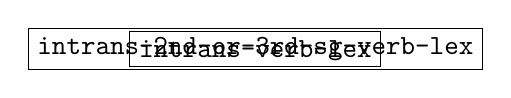
\begin{tikzpicture}
        \Tree  [.\texttt{lex-item} \edge[dashed];
               [.\texttt{verb-lex} \edge[dashed];
               [.\texttt{main-verb-lex};
                  [.\texttt{intransitive-verb-lex}
                    [.\texttt{nom-intransitive-verb-lex}
                    [. \node[draw] {\texttt{intrans-verb-lex}};
                    %   \edge[thick];
                    [. \node[draw] {\texttt{intrans-2nd-or-3rd-sg-verb-lex}}; ] ] ] ] ]
                \edge[dashed];
                [.\texttt{transitive-verb-lex} ] ] ]
                % ]
    \end{tikzpicture}
    } % attop
\end{exe}

Turning now to phrase structure rules -- at this stage, the grammar of \sclera\
uses the same basic rule types as defined by the grammar of Dutch. The three
most important correspond to the `schemata' of canonical \hpsg
\citep{pollard1994head}. Provided as entries in \texttt{rules.tdl}, as shown in
\cref{ex:sclera:rulestdl}, these types instantiate the backbone for the SVO
order assumed of \sclera\ strings in the previous section.

\begin{exe}

    \ex\label{ex:sclera:rulestdl}Top of \texttt{rules.tdl}\\
    \begin{verbatim}
head-comp := head-comp-phrase. ;; (1)
subj-head := subj-head-phrase. ;; (2)
head-spec := head-spec-phrase. ;; (3)
    \end{verbatim}
\end{exe}

Word order is accounted for by combining rule types that impart unique
`headedness' to the daughters of a phrase with rules that constrain the linear
position of the head daughter in relation to her non-head sisters. For
instance, the \emph{head-complement phrase} rule, in
\cref{ex:sclera:rule:headcomp}, combines the constraints of
\emph{basic-head-1st-comp-phrase} (a subtype of `dominance' rule types
involving complements) with the constraints belonging to the type
\emph{head-initial}, which, as its name suggests, requires that the head
daughter come first in the phrase. Variations on this logic are used in the
type definitions of the other two rules, except here the head daughter is
required, by \emph{head-final}, to come last, or -- as these rules are
consistently binary (see \cref{par:naryvsbinary}) -- second.

\begin{exe}
    \ex\label{ex:sclera:rule:headcomp}
\begin{verbatim}
head-comp-phrase := basic-head-1st-comp-phrase & head-initial.
\end{verbatim}
    \ex\label{ex:sclera:rule:subjhead}
\begin{verbatim}
subj-head-phrase := decl-head-subj-phrase & head-final &
    [ HEAD-DTR.SYNSEM.LOCAL.CAT.VAL.COMPS < > ].
\end{verbatim}
    \ex\label{ex:sclera:rule:headspec}
\begin{verbatim}
head-spec-phrase := basic-head-spec-phrase & head-final.
\end{verbatim}
\end{exe}

The result of the customization stage (followed by a fair amount of manual
intervention) is a partial model of \sclera\ comprising, among other, type
descriptions for simplex `noun' and `verb' pictographs and basic grammar rules
for phrase construction (which, it ought to be mentioned, also implement the
semantic composition principles of \hpsg\ \citep{sag1999syntactic}) as well as
the internal structure of phrases, with respect to both linear precedence and
immediate dominance \citep{pollard1994head}. However, the current model is not
entirely ready to be used for parsing yet. The next section aims to fix this.

\subsection{`Bringing back' determiners}
\label{sub:MissingDeterminers}

Recall that the function of the grammar of \sclera\ within the \depicto\ system
is to `extract' as much semantic information as possible from the pictographic
input, which, by natural language standards, is vastly underspecified. In order
to do this, then, the grammar must be able to make hypotheses about semantic
structure based on what little clues the input affords. The grammar developed
so far does not do this, however; only the immediate surface structure of the
input is taken into account. As a result, the absence of determiners in the
\sclera\ language causes the grammar to run into trouble. This is because of
two reasons. First, on a theoretical level, the \lingo\ Matrix incorporates the
assumption that the referential indices, i.e., `noun' predications, of a
well-formed \mrs\ must always be outscoped by some quantifier
\citep{copestake2005minimal}. Second, in the grammar of Dutch, from which the
grammar of \sclera\ derives its types, this assumption is worked out by an
interplay of constraints which have the effect of requiring that common nouns
select for an obligatory `specifier' (quantifier/determiner). This is what is
specified by the negative value of the \textsc{opt} attribute in the AVM
description of the type \emph{common-noun-lex} in \cref{ex:sclera:common-noun},
the relevant portion of which is repeated here in
\cref{ex:sclera:featurepath:opt-}. Since determiners do not occur on the input,
the parser fails when passed a \sclera\ string containing pictographs of the
`common noun' type.

\begin{exe}
    \ex\label{ex:sclera:featurepath:opt-}
    \begin{avm}
        [ \asort{common-noun-lex}
           synsem|local|cat|cal|spr &  < [ local|cat|head & det \\
                                        opt \; \textnormal{-} ] > ]
    \end{avm}
\end{exe}

However, not all types of nouns select an explicit determiner, as
\cref{ex:mass-noun} and \cref{ex-pronoun} show for mass nouns and pronouns,
respectively. These types take either no specifier or take one but mark it as
optional.

\begin{exe}
    \ex\label{ex:mass-noun}
            \textbf{Water} has three forms.
    \ex\label{ex-pronoun}
            \textbf{You} should tell \textbf{me} about \textbf{them}.
\end{exe}

When occurring without a specifier, as in the examples above, these noun types
form so-called \emph{bare noun phrases}. However, semantically, their
referential indices are still scoped by an `exist' quantifier, as represented
semi-formally in \cref{ex:exist-noun}.

\begin{exe}
    \ex\label{ex:exist-noun}
    $ exists(x, noun\_relation(x) )$
\end{exe}

In order to achieve this effect, the \lingo\ Matrix provides a definition of a
unary phrase rule type that takes a single nominal head daughter with an
optional specifier constraint and \emph{adds} a quantification relation to the
list of \emph{elementary predications} provided by the head daughter. The
semantic contribution of the rule is specified on the attribute \textsc{c-cont}
(\emph{Construction CONTent}). As the identity statements (prefixed by a
`\textsc{\#}') in the \tdl\ description in \cref{ex:dutch:bare-np-phrase:verb}
show, the \textsc{c-cont} part of the rule identifies the daughter's
\emph{index} with the index argument (\textsc{arg0}) of \emph{quant-relation}.
At the same time time, via identity with an attribute of the handle constraint
relation in \textsc{hcons}, the top handle (\textsc{ltop}) of the daughter is
placed within the quantifier's scope.

\begin{exe}
    \ex\label{ex:dutch:bare-np-phrase:verb}
    {\small
    \begin{verbatim}
basic-bare-np-phrase := head-only &
  [ SYNSEM.LOCAL.CAT.VAL [ SPR < >,
               SUBJ < >,
               COMPS < >,
               SPEC < > ],
    HEAD-DTR.SYNSEM.LOCAL [ CAT [ HEAD noun,
                                  VAL [ SPR < [ LOCAL.CAT.HEAD det,
                                                OPT + ] >,
                                        SUBJ < >,
                                        COMPS < > ] ],
                            CONT.HOOK [ INDEX #index,
                                        LTOP #larg ] ],
    C-CONT [ RELS <! quant-relation &
                        [ ARG0 #index,
                          RSTR #harg ] !>,
             HCONS <! qeq &
                       [ HARG #harg,
                         LARG #larg ] !>,
             ICONS <! !>,
             HOOK [ INDEX #index ] ] ].
    \end{verbatim}
    }
\end{exe}

The Matrix definition of the rule leaves the specification of the quantifier's
\textsc{pred} value (i.e., relation name) to the precise grammar in which it is
used. In the grammar of \sclera\ this becomes \emph{`exist\_q\_rel'}, as shown in \cref{ex:sclera:bare-np:verb}.

\begin{exe}
    \ex\label{ex:sclera:bare-np:verb}
    {\small
    \begin{verbatim}
bare-np-phrase := basic-bare-np-phrase &
  [ C-CONT.RELS <! [ PRED 'exist_q_rel' ]  !> ].
    \end{verbatim}
    }
\end{exe}

Example \cref{ex:sclera:bare-np:tree} shows the \emph{basic-np-phrase} rule
being used to parse the mass noun \emph{water} (as it is used
\cref{ex:mass-noun}). Notice that the mother node, i.e., the value of the
top-level feature path \textsc{synsem|local}, is (a) a saturated noun phrase
(NP), which makes the resulting structure compatible with the head-complement
and head-subject rules; and (b) that its relations list (under \textsc{cont})
is the append of those of \textsc{c-cont} and \textsc{head-dtr}. In short, the
semantic content of the mother node, or, as it were, the `left side' of the
phrase rule, contains \emph{more} than what is found on the actual input.

\begin{exe}
    \ex\label{ex:sclera:bare-np:tree}
    \avmoptions{notactive}
    \tikzset{every tree node/.style={align=center,anchor=north}}
    \tikzset{level 1/.style={level distance=320pt}}
    \tikzset{level 2/.style={level distance=180pt}}
    \attop{\begin{tikzpicture}
    % [level distance=250pt]
\Tree [ .NP\\{
    \begin{avm}
\[ \asort{bare-np-phrase}
   synsem\|local & \[ cat\|val\|spr \; <\;> \\
                      cont \; \[ hook\|index \; \@2  \\
                                 rels  \; \@5 $\oplus$ \@4 \]  \] \\
   c-cont & \[ hook\|index \; \@2 \\
               rels \; \@5 \< \[ pred & \avmstring{exist\_q\_rel} \\
                                 arg0 & \@2  \\
                                 rstr & \@6 \]  \>  \\
               hcons \; \< \[ \asort{qeq}
                              harg & \@6 \\
                              larg & \@3 \] \> \] \\
   head-dtr \; \@1 \]
     \end{avm} }
        [ .N\\{
\begin{avm}
\@1 \[ synsem\|local & \[ cat\|val\|spr \; \< \[ local\|cat\|head & det \\
                                            opt \; \textnormal{+} \] \> \\
                         cont \; \[ hook & \[ index & \@2 \\
                                             ltop & \@3 \] \\
                                   rels & \@4 \< \[ pred &
                                            \avmstring{\_water\_n\_rel}  \]
                                               \> \] \] \]
\end{avm} }
           water ] ]
        \end{tikzpicture}
        } % attop
\end{exe}

This notion that a phrase rule can itself \emph{contribute} semantic
information (or simply modify it) forms the basis for many of the analyses
which enable the \sclera\ grammar to make the best of its semantically
impoverished input, including the grammar's treatment of missing determiners.
(In fact, if the foregoing explanation is at all clear, the reader may by now
already have some idea as to how this might work.) All that is needed to `bring
back' determiners is a slightly modified version of the \emph{bare-np-phrase}
rule which unifies with common nouns, i.e., noun entries with a
\emph{non-optional} specifier constraint, and places these nouns in a similar
scoping relation. The \emph{bare-np-phrase} rule, therefore, is copied and
modified accordingly to obtain the \tdl\ description in
\cref{ex:sclera:sclera-basic-insert-det-rule:verb}. Notice that, instead of
`exist\_q\_rel', this rule contributes a new quantifier relation,
`q\_rel\_min'. Though specified as a string in the \sclera\ grammar, this
quantifier relation is later converted to a type, which, as the next chapter
will explain in more detail, is situated at the top of a local hierarchy of
different determiner and quantifier relations. Slightly ahead of time (the
hierarchy is the domain of the target grammar), this hierarchy of determiner
types is shown in \cref{ex:dutch-sclera:quantifier-types:tree}). By virtue of
the \emph{sclera-basic-insert-det} rule, the \sclera\ grammar can now parse
strings containing common nouns without requiring that these be accompanied by
(non-existent) determiners.


\begin{exe}
    \ex\label{ex:sclera:sclera-basic-insert-det-rule:verb}
    {\small
    \begin{verbatim}
sclera-basic-insert-det-rule := head-only &
  [ SYNSEM.LOCAL.CAT.VAL [ SPR < >,
                           SUBJ < >,
                           COMPS < >,
                           SPEC < > ],
    HEAD-DTR.SYNSEM.LOCAL [ CAT [ HEAD noun,
                                  VAL [ SPR < [ LOCAL.CAT.HEAD det,
                                                OPT - ] >,
                                        SUBJ < >,
                                        COMPS < > ] ],
                            CONT.HOOK [ INDEX #index,
                                        LTOP #larg ] ],
    C-CONT [ RELS <! quant-relation &
                      [ PRED "q_rel_min",
                        ARG0 #index,
                        RSTR #harg ] !>,
             HCONS <! qeq &
                      [ HARG #harg,
                        LARG #larg ] !>,
             ICONS <! !>,
             HOOK [ INDEX #index,
                    LTOP #larg ] ] ].
    \end{verbatim}
    }
\end{exe}


\begin{exe}
    \ex\label{ex:dutch-sclera:quantifier-types:tree}
    \tikzset{every tree node/.style={align=center,anchor=north}}
    \attop{
    \emph{
    \begin{tikzpicture}
        \Tree [.predsort
                [.q\_rel\_min
                   def\_q\_rel\\{\textnormal{(definite determiner)}}
                   indef\_q\_rel\\{\textnormal{(indefinite determiner)}}
                   exist\_q\_rel\\{\textnormal{(`exists' relation)}} ] ]
    \end{tikzpicture}
    } % emph
    } % attop
\end{exe}

The parse of \sclera\ `dog', represented as a tree diagram in
\cref{ex:sclera:insert-det-rule:tree}, is clearly similar to that licensed by
the rule upon which it is based. In fact, the differences are hard to spot. Yet
the importance of the \emph{sclera-insert-det-rule} for the grammar of \sclera\
cannot be overstated.

\begin{exe}
    \ex\label{ex:sclera:insert-det-rule:tree}
    \avmoptions{notactive}
    \tikzset{every tree node/.style={align=center,anchor=north}}
    \tikzset{level 1/.style={level distance=320pt}}
    \tikzset{level 2/.style={level distance=180pt}}
    \attop{\begin{tikzpicture}
    % [level distance=250pt]
\Tree [ .NP\\{
    \begin{avm}
\[ \asort{sclera-basic-insert-det-rule}
   synsem\|local & \[ cat\|val\|spr \; <\;> \\
                      cont \; \[ hook\|index \; \@2  \\
                                 rels  \; \@5 $\oplus$ \@4 \]  \] \\
   c-cont & \[ hook\|index \; \@2 \\
               rels \; \@5 \< \[ pred & \avmstring{q\_rel\_min} \\
                                 arg0 & \@2  \\
                                 rstr & \@6 \]  \>  \\
               hcons \; \< \[ \asort{qeq}
                              harg & \@6 \\
                              larg & \@3 \] \> \] \\
   head-dtr \; \@1 \]
     \end{avm} }
        [ .N\\{
\begin{avm}
\@1 \[ synsem\|local & \[ cat\|val\|spr \; \< \[ local\|cat\|head & det \\
                                            opt \; \textnormal{-} \] \> \\
                         cont \; \[ hook & \[ index & \@2 \\
                                             ltop & \@3 \] \\
                                   rels & \@4 \< \[ pred &
                                            \avmstring{\_dog\_n\_rel}  \]
                                               \> \] \] \]
\end{avm} }
           \includegraphics[width=2cm]{sclera/hond1} ] ]
        \end{tikzpicture}
        } % attop
\end{exe}

With the \emph{sclera-insert-det-rule} in place, the grammar can now parse
simple \sclera\ strings of the kind shown in \cref{ex:sclera:dog-see-bus},
repeated for convenience here by \cref{ex:sclera:dog-see-bus1}. The tree
diagram representation of the parse is given in
\cref{ex:sclera:dog-see-bus:tree}.

\begin{exe}
    \ex \label{ex:sclera:dog-see-bus1}\attop{
    \gll
       {\includegraphics[width=2cm]{sclera/hond3}\hspace{0.5cm}}
       {\includegraphics[width=2cm]{sclera/zien}\hspace{0.5cm}}
       {\includegraphics[width=2cm]{sclera/bus}} \\
       \emph{dog} \emph{see} \emph{bus} \\
    }
\end{exe}


\begin{exe}
    \ex\label{ex:sclera:dog-see-bus:tree}
    \tikzset{every tree node/.style={align=center,anchor=north}}
        \tikzset{level 3/.style={level distance=30pt}}
    \attop{
    \begin{tikzpicture}[level distance=50pt]
        \Tree [.S\\{\emph{head-subject rule}}
                   [.NP\\{\emph{sclera-det-insert rule}}
                       [.N {`dog'} ] ]
                   [.VP\\{\emph{head-complement rule}} [ .V {`see'} ]
                    .NP\\{\emph{sclera-det-insert rule}} [ .N {`bus'} ] ] ]
    \end{tikzpicture}
    }
\end{exe}

\section{Understanding the \mrs\ output}
\label{sec:sclera:mrsoutput}

When using the \ace\ processor \citep{sweaglesACE}, the output of parsing is a
\emph{plain-text} \mrs\ representation. An example of such an \mrs\
representation is given in \cref{ex:sclera:outputofparsing:text}, which shows
the fully semantic structure to which the string in
\cref{ex:sclera:dog-see-bus:tree} resolves, i.e., the semantic information
found at the root node `S'.

\begin{exe}
    \ex\label{ex:sclera:outputofparsing:text} Output \mrs\ representation of `dog see bus'\\
    \scriptsize
    \begin{verbatim}
SENT: dog see bus
[ LTOP: h0
  INDEX: e2 [ e SF: prop-or-ques E.TENSE: tense E.ASPECT: aspect E.MOOD: mood ]
  RELS: < [ "_dog_n_rel"<-1:-1> LBL: h4 ARG0: x3 [ x PNG.PER: person
                                                     PNG.NUM: number
                                                     PNG.GEND: gender ] ]
          [ "q_rel_min"<-1:-1> LBL: h5 ARG0: x3 RSTR: h6 BODY: h7 ]
          [ "_see_v_rel"<-1:-1> LBL: h1 ARG0: e2 ARG1: x3 ARG2: x8 [ x PNG.PER: person
                                                                       PNG.NUM: number
                                                                       PNG.GEND: gender ] ]
          [ "_bus_n_rel"<-1:-1> LBL: h9 ARG0: x8 ]
          [ "q_rel_min"<-1:-1> LBL: h10 ARG0: x8 RSTR: h11 BODY: h12 ] >
  HCONS: < h0 qeq h1 h6 qeq h4 h11 qeq h9 > ]
    \end{verbatim}
\end{exe}

Although the representation in the example has been slightly simplified (and
beautified with extra indentation), it may be observed that its general format
approximates that of the AVM diagram given in \cref{sub:mrs}. However, there
are also some differences. The attributes \textsc{ltop} and \textsc{index} are
taken out of the \textsc{hook} feature and promoted to the top level of the
representation, and, presumably for legibility, the \emph{qeq} constraints are
not presented as individual feature structures, nor are they separated by a
comma. More salient, however, is the appearance of attribute-value pairs such
as \texttt{E.TENSE: tense} and \texttt{PNG.GEND: gender} after referential
variables (e.g., \texttt{x8}) and event variables (e.g., \texttt{e2}). These
convey additional semantic properties associated with the values of the
attributes \textsc{index} or \textsc{arg0}. In example
\cref{ex:sclera:outputofparsing:text}, all but one are left underspecified: the
value of \texttt{SF} (third line from the top) conveys that the illocutionary
force of the parsed string is either declarative or interrogative. When the
parsed string contains pronouns, however, the properties of the referential
index/variable are more specific, as the fragment in \cref{ex:sclera:outputofparsing:I} shows. The referential (`\texttt{ARG0}') argument of the predicate `\_pronoun\_n\_rel' has the property of being first person singular (\emph{I} in English), but leaves the value of the \texttt{GEND} property underspecified, since it is gender-neutral.

\begin{exe}
    \ex\label{ex:sclera:outputofparsing:I} Fragment of \mrs\ representation of `I walk'\\
    \scriptsize
    \begin{verbatim}
RELS: < [ "_pronoun_n_rel"<-1:-1> LBL: h4 ARG0: x3 [ x PNG.PER: 1st
                                                       PNG.NUM: singular
                                                       PNG.GEND: gender ] ]
    \end{verbatim}
\end{exe}

\section{Extending the \sclera\ grammar}
\label{sec:casestudies}

This section presents three case studies which extend the grammar of \sclera\
developed in the previous section and, in so doing, offer some indication,
albeit tentative, of the practicability of a rule-based approach to modelling
\sclera\ as a language in its own right. \cref{subs:cs:temp-disambig} and
\cref{subs:cs:interrogative} introduce two new phrase rules that demonstrate
how the semantic accuracy of the grammar can be enhanced so that it can
distinguish, on the one hand, between past and `other' tense readings of the
input and, on the other hand, between declarative and illocutionary readings.
Abstractly, both phrase rules function by identifying a specific non-head
daughter `particle' and modifying the semantic content of the head daughter to
match some feature contributed by this `particle'. (Such particles can also be
thought of as `indicators' or `operators'. In part-of-speech terms, they
correspond to adverbs, though there are some differences in overall function.)
Moving on, the third case study (\cref{subs:cs:complex-pictos}) details a first
attempt at extending the grammar's coverage to conceptually complex
pictographs. I say `first attempt' because (a) only a selection of complex
pictograph types has so far been incorporated; (b) the local type hierarchy
which they deploy is fairly rudimentary; and (c) as a result, the division of
labor between the lexicon and the type hierarchy is currently biased toward the
lexicon. Nevertheless, the discussion in this section demonstrates that complex
pictographs \emph{can} in principle be incorporated, provided that a handful of
new rules and two new additions to the feature geometry are introduced.

\subsection{Temporal disambiguation} %  with adverbial pictos
\label{subs:cs:temp-disambig}

\sclera\ `verbs' are underspecified for tense. As a result, the clause
structures which they project allow as many readings as there are tenses
available in the semantic universe. Thus, supposing a minimal theory of tense
types, the string in \cref{ex:sclera:dog-see-bus1} can correspond, among other,
to the three different readings shown in \cref{ex:temp:readingsbasic1}, all
other sources of underspecification kept equal.

\begin{exe}
    \ex\label{ex:temp:readingsbasic1} `dog see bus' $ \Leftrightarrow $
    \begin{xlist}
        \ex `The dog \emph{sees} the bus.' (Present tense domain)
        \ex `The dog \emph{saw} the bus.' (Past tense domain)
        \ex `The dog \emph{will} see the bus.' (Future tense domain )
    \end{xlist}
\end{exe}

Similar to the `re-introduced' determiner relation in
\cref{sub:MissingDeterminers}, which, as we saw there, is actually a
generalization over several concrete kinds of determiners, the \emph{intended}
tense of a simple string such as `dog see bus' is grammatically undecidable,
and is therefore best left underspecified. It is arguably a limitation of the
\sclera\ set that it does not contain pictographs which explicitly specify the
intended tense. However, the set does contain a number of pictographs that
depict temporal concepts and which can conceivably function as adjuncts of time
in a \sclera\ clause. A selection is given by \cref{ex:temp:pictosoftime}.

\begin{exe}
    \ex
    \label{ex:temp:pictosoftime}
    \attop{
    \gll
    {\includegraphics[height=2cm]{sclera/gisteren}\hspace{0.2cm}}
    {\includegraphics[height=2cm]{sclera/vandaag}\hspace{0.2cm}}
    {\includegraphics[height=2cm]{sclera/nu}\hspace{0.2cm}}
    {\includegraphics[height=2cm]{sclera/morgen}}\\
    {`yesterday'} {`today'} {`now'} {`tomorrow'}\\
    } % attop
\end{exe}

In natural language, such time adjuncts are generally appropriate to a single
specific temporal domain. As \cref{ex:temp:read/w/yest} illustrates for
`yesterday', the effect in \sclera\ is that they restrict the felicitousness of
individual tense readings.

\begin{exe}
    \ex\label{ex:temp:read/w/yest} `dog see bus yesterday'
        $ \Leftrightarrow $
    \begin{xlist}
        \ex[]{`The dog \emph{saw} the bus yesterday.'}
        \ex[*]{`The dog \emph{sees} the bus yesterday.'}
        \ex[*]{`The dog \emph{will} see the bius yesterday.'}
    \end{xlist}
\end{exe}

From a procedural perspective, these adjuncts can be understood as
\emph{modifying} the tense of the verb phrase with which they combine so that
its tense is constrained to a specific type. This behavior is modelled by the
introduction of a new phrase rule type called
\textbf{\emph{temp-adverb-verb-phrase}} (the adjuncts of time in
\cref{ex:temp:pictosoftime} are analysed as simple adverbs here). As its \tdl\
description shows, this rule belongs to the `head-modifier' category
\citep{pollard1994head}. Essentially, it identifies the \textsc{tense} value of
the index of its non-head daughter, which must be an adverb\footnote{In \hpsg,
adverbs are treated semantically as `events' \citep{pollard1994head}}, with the
\textsc{tense} value of the index of \textsc{c-cont}. The index of this last
feature is passed up to the mother of the rule through constraints inherited
from its supertypes. While \textsc{c-cont} shares its \textsc{tense} value with
the adverbial daughter, all features found under \textsc{c-cont}'s
\textsc{hook} attribute are shared with those of the head daughter, including
the \textsc{tense} attribute. By virtue of unification, however, the compatible
yet more specific value of the non-head daughter's \textsc{tense} feature
`wins', as it were, over the more general value of the head-daughter's
\textsc{tense} feature. For the time being, finally, the rule requires the head
daughter to be a finite clause, specified by \texttt{[ CAT.MC + ]}. This goes
against conventional wisdom, which analyzes adjuncts as modifying the verb
phrase, not the clause as a whole, and should probably be revised later on.

\begin{exe}
    \ex\label{ex:temp:temp-phrase:verb}
    {\small
    \begin{verbatim}
temp-adverb-verb-phrase := basic-head-mod-phrase-simple &
                                head-initial & isect-mod-phrase &
  [ C-CONT.HOOK #hook & [ INDEX.E.TENSE #tense ],
    NON-HEAD-DTR.SYNSEM.LOCAL [ CAT.HEAD adv,
                                CONT.HOOK.INDEX.E.TENSE #tense ],
    HEAD-DTR.SYNSEM.LOCAL [ CONT.HOOK #hook,
                            CAT.MC + ] ].
    \end{verbatim}
    }
\end{exe}

As the tree representation of the parse of the string `dog see bus
yesterday' in \cref{ex:temp:temp-adv-verb:tree} shows, the effect of the
\emph{temp-adverb-verb-phrase} rule is that the adjunct of time `imparts' its
\textsc{tense} constraint to the clause/verb phrase which it modifies.

\begin{exe}
    \ex\label{ex:temp:temp-adv-verb:tree}
    \avmoptions{notactive}
    \avmhskip{0.5em}
    \tikzset{every tree node/.style={align=center,anchor=base}}
    \tikzset{level 1/.style={level distance=160pt}}
    \tikzset{level 2/.style={level distance=120pt}}
    % \tikzset{level 3/.style={level distance=40pt}}
    \attop{
    \noindent
    \begin{tikzpicture}
    % [level distance=250pt]
\Tree [ .S\\{
    \begin{avm}
\[ \asort{temp-adverb-verb-phrase}
   synsem\|local & \[ cat\|head & verb \\
                      cont\|hook & \@1 \] \\
   c-cont\|hook & \@1 \[ index\|e\|tense & \@3 \] \\
   head-dtr & \@2 \\
   non-head-dtr & \@4 \]
    \end{avm}}
          [ .S\\{
          \begin{avm}
\@2 \[ cat \; \[ head & verb \\
                mc & \textnormal{+} \] \\
       cont\|hook \; \@1 \[ index\|e\|tense & tense \] \]
          \end{avm}}
                \edge[roof]; {`dog see bus'} ]  % left ]
          [ .Adv\\{  % right
                \begin{avm}
\@4 \[ \asort{temporal-adjunct-picto}
       cat\|head \; \[ \asort{adverb}
                  mod & \< \@2 \> \]  \\
          cont\|hook\|index\|e\|tense & \@3 past \]
                \end{avm}}
                `yesterday' ] ]
        \end{tikzpicture}
        } % attop
\end{exe}

Just like the rule responsible for the `re-introduction' of determiners, the
\emph{temp-adverb-verb-phrase} rule offers a means of enriching the semantic
structure that is extracted from the input string during parsing. Later on in
the translation process (in the generation stage, to be specific), the
resulting increase in specificity will amount to increased accuracy. Itself
still a proof of concept, the rule is not as `strict' as it should be: it is
not constrained to time adjuncts \emph{only}. However, since the grammar
currently models only one adverb and this adverb is the time adjunct
`yesterday', this does not pose any problems at the moment. To be clear,
however, adding the remaining time adjunct pictos listed in
\cref{ex:temp:pictosoftime} to the grammar would be a relatively simple task.

Finally, the \emph{temp-adverb-verb-phrase} rule exhibits two limitations that
will need to be overcome if it is to be useful in a real-life context. The
first is that the head daughter is required to come \emph{before} the modifying
daughter and that this head daughter needs to be a finite clause. Ignoring the
second issue, the restriction on word order prevents even simple variations on
the string in \cref{ex:temp:read/w/yest} from being accepted by the grammar:
e.g., `yesterday dog see bus'. The second main limitation is that the rule
incorporates no `claims' about aspect. Thus, `dog see bus now', though
appropriately interpreted in the present tense, allows both the continuous
reading `\texttt{?} the dog is seeing the bus now' and the more bounded, simple
present reading `the dog sees the bus now'. The decidedly odd character of the
continuous reading is difficult to dismiss, though it is possible that this is
something that might need to be assigned to a different component of the
grammar, one that deals with, say, pragmatics, for instance.

\subsection{Triggering the interrogative mood} % yes-no questions
\label{subs:cs:interrogative}

As shown by the \mrs\ output of parsing `dog see bus' in
\cref{ex:sclera:outputofparsing:text}, the relevant portion of which is
repeated below in \cref{ex:interr:MRS:verb}, \sclera\ clauses are by default
also underspecified for illocutionary force, or \emph{mood}.

\begin{exe}
    \ex\label{ex:interr:MRS:verb}
    \begin{verbatim}
... INDEX: e2 [ e SF: prop-or-ques ...
    \end{verbatim}
\end{exe}

The value of the \textsc{sf} (\emph{Sentence Force}) property of the event
variable, viz., \emph{prop-or-ques}, indicates that the clause may be either a
proposition or a question, these two options corresponding to the declarative
and interrogative mood, respectively. As a result, the clause `dog see bus'
allows both readings in \cref{ex:interr:readingsbasic1} -- again, all other
sources of underspecification kept equal.

\begin{exe}
    \ex\label{ex:interr:readingsbasic1} `dog see bus' $ \Leftrightarrow $
    \begin{xlist}
        \ex `The dog sees the bus.' (Declarative mood)
        \ex `Does the dog see the bus?' (Interrogative mood)
    \end{xlist}
\end{exe}

In a real use context, such unrestrained alternation between, interactively,
two very different readings would probably cause some confusion. Therefore, the
default reading is constrained to the declarative mood. (In the current version
of the system, this constraint is contributed by the target grammar, so it is
discussed later.) Nevertheless, there is no reason to assume that a
hypothetical user might not at some point want to use the system to ask a
question. In fact, despite the comparatively higher frequency of the
declarative mood, this is almost inevitable. The grammar should provide some
means, therefore, of `sensing' when the intended reading concerns the
interrogative mood.

The \sclera\ set contains a small set of pictographs which depict literal
punctuation marks. Two such symbols are given in \cref{ex:sclera:punctuation}.
(The exclamation mark is provided on account of its possible association with
the imperative mood.)

\begin{exe}
    \ex \label{ex:sclera:punctuation}\attop{
    \gll
       {\includegraphics[width=2cm]{sclera/vraagteken}\hspace{0.5cm}}
       {\includegraphics[width=2cm]{sclera/uitroepteken}\hspace{0.5cm}}\\
       {`question'} {`exclamation'}\\
    }
\end{exe}

Assuming that users can be taught to associate a `question mark' symbol with
the interrogative mood, using it as a sort of explicit mood marker, the string
in \cref{ex:interr:readings2} only has one appropriate reading, namely, as
having interrogative illocutionary force.

\begin{exe}
    \ex\label{ex:interr:readings2} `dog see bus question' $ \Leftrightarrow $
    \begin{xlist}
        \ex[]{`Does the see the bus?'}
        \ex[*]{`The dog sees the bus.'}
    \end{xlist}
\end{exe}

Thus, just as the time adjunct `yesterday' in \cref{subs:cs:temp-disambig}
\emph{triggers} the past tense, so the illocution operator `question' can be
interpreted as triggering the interrogative mood. This `triggering' behavior is
modelled by a new rule which, based on the same basic mechanism as the
\emph{temp-adverb-verb-phrase} rule in \cref{subs:cs:temp-disambig}, identifies
the illocutionary force value (found on the feature path
\textsc{synsem|local|cont|hook|index|sf|}) of a verbal head daughter with the
more specific illocutionary force value of the operator `question', which
serves as the non-head daughter.

For the current purposes, the illocution operator `question' could be treated
as an adverb. However, since its function does not really have an equivalent in
natural language, where the question mark is generally categorized under the
orthographic domain, it is added to the grammar as a new lexical type called
\emph{question-picto}. As the partial AVM description in
\cref{ex:interr:ques-pic:avm} shows, this type modifies a single saturated
verb-headed feature structure and bears an \textsc{sf} (illocutionary force)
feature with the value \emph{ques} (a subtype of \emph{prop-or-ques}). Note,
however, that its \textsc{rels} list is empty: it does not contribute a
predicate relation. Finally, the type bears a newly posited \textsc{head} value
\emph{ques-mod}, which itself is introduced to the type hierarchy as a subtype
of a new head type \emph{iforce-mod}, as \cref{ex:interr:ques-mod:typeh} shows.

\begin{exe}
    \ex\label{ex:interr:ques-pic:avm}
    \avmoptions{notactive}
    \avmhskip{0.5em}
    \begin{avm}
\[ \asort{question-picto}
   synsem\|local & \[ cat\|head & \[ \asort{ques-mod}
                 mod & \< \[ local\|cat & \[ head & verb\\
                                 val & \[ subj \; \textnormal{<\;>} \\
                                        comps \; \textnormal{<\;>} \] \]
                        \> \] \] \\
                      cont & \[ hook\|index\|sf & ques \\
                                rels \; \textnormal{<\;>} \] \] \]
    \end{avm}
\end{exe}

\begin{exe}
    \ex\label{ex:interr:ques-mod:typeh}
    \tikzset{every tree node/.style={align=center,anchor=base}}
    \attop{
    \emph{
    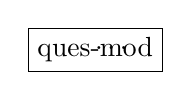
\begin{tikzpicture}
        \Tree [.head
                [.iforce-mod
                   [. \node[draw]{ques-mod}; ] ]
               \edge[dashed]; verb
               \edge[dashed]; noun
               \edge[dashed]; \textnormal{[$\ldots$]} ]
    \end{tikzpicture}
    } % emph
    } % attop
\end{exe}

The rule type that is introduced to enables this new lexical type to combine
with the structure on its \textsc{mod} list is called the
\textbf{\emph{modify-illocution-phrase}} rule. Its \tdl\ description is given
in \cref{ex:interr:phraserule:tdl}. Similar to the
\emph{temp-adverb-verb-phrase} type in \cref{subs:cs:temp-disambig}, it is
essentially a head-modifier rule \citep{pollard1994head} that stipulates a
structure sharing constraint between a property of the index of the mother node
and the same property of the index of the non-head daughter. Its definition
differs from that of the \emph{temp-adverb-verb-phrase} type in that
it states no explicit identity relation between the \textsc{hook} path of the
head daughter and the \textsc{hook} path of the mother, and that it explicitly
specifies that the \textsc{rels} under \textsc{c-cont} is empty. The first
difference is due to the fact that the \textsc{hook} constraint is already
covered by constraints inherited from the \emph{head-compositional} phrase
type. The empty \textsc{rels} list is a feature which ensures that the rule
type is compatible with the mechanisms of semantic composition defined in the
Matrix type hierarchy.

\begin{exe}
    \ex\label{ex:interr:phraserule:tdl}
    {\small
    \begin{verbatim}
modify-illocution-phrase := basic-head-mod-phrase-simple &
                                  head-initial & head-compositional &
    [ C-CONT [ HOOK.INDEX.SF #illocution,
               RELS <! !> ],
      HEAD-DTR.SYNSEM.LOCAL [ CAT.MC + ],
      NON-HEAD-DTR.SYNSEM.LOCAL [ CAT.HEAD ques-mod,
                                  CONT.HOOK.INDEX.SF #illocution ] ].
    \end{verbatim}
    }
\end{exe}

An example of how the \emph{modify-illocution-phrase} rule is used to analyse
the string `dog see bus question' is given in
\cref{ex:interr:mod-ill-phr:tree}.

\begin{exe}
    \ex\label{ex:interr:mod-ill-phr:tree}
    \avmoptions{notactive}
    \avmhskip{0.5em}
    \tikzset{every tree node/.style={align=center,anchor=base}}
    \tikzset{level 1/.style={level distance=170pt}}
    \tikzset{level 2/.style={level distance=130pt}}
    % \tikzset{level 3/.style={level distance=40pt}}
    \attop{
    \noindent
    \begin{tikzpicture}
    % [level distance=250pt]
\Tree [ .S\\{
    \begin{avm}
\[ \asort{modify-illocution-phrase}
   synsem\|local & \[ cat\|head & verb \\
                      cont\|hook & \@1 \] \\
   c-cont & \[ hook & \@1 \[ index\|sf & \@3 \] \\
               rels & \textnormal{< >} \] \\
   head-dtr & \@2 \\
   non-head-dtr & \@4 \]
    \end{avm}}
          [ .S\\{
          \begin{avm}
\@2 \[ cat \; \[ head & verb \\
                mc \; \textnormal{+} \] \\
       cont\|hook \; \@1 \[ index\|sf & tense \] \]
          \end{avm}}
                \edge[roof]; {`dog see bus'} ]  % left ]
          [ .O(perator)\\{  % right
                \begin{avm}
\@4 \[ \asort{question-picto}
       cat\|head \; \[ \asort{ques-mod}
                  mod & \< \@2 \> \]  \\
          cont\|hook\|index\|sf & \@3 ques \]
                \end{avm}}
                `question' ] ]
        \end{tikzpicture}
        } % attop
\end{exe}

Like the \emph{temp-adverb-verb-phrase} rule, this new addition represents a
step in the direction of modelling \sclera\ as a system with its own rules.
Just as, in natural language, a rising tone contour generally signals a
question (in non-tone languages, at least) the `question' pictograph serves as
a contextual marker of the interrogative mood and, as such, is treated as a
part of the grammar. The significance for \depicto\ as an assisitve writing
tool is an overall increase in expressivity -- provided that users are able to
recognize the interactional contribution of the `question' pictograph. As with
much of the work discussed in this chapter, the purpose of the rule presented
here is primarily to offer an early indication of the practicability of a
rule-based approach to modelling \sclera. Thus, although it works fine in its
current function, the \emph{modify-illocution-phrase} rule is still in an
experimental stage. As a result, there are some limitations. In the first
place, it only supports \emph{polar} interrogatives, i.e., yes-no questions.
\emph{Wh}-questions, which could be formulated using the \sclera\ symbols in
\cref{ex:sclera:wh-elements} (these symbols each have a number of variants),
should at some point be covered by the model, although, admittedly, such
questions types probably warrant a different rule altogether.

\begin{exe}
    \ex \label{ex:sclera:wh-elements}\attop{
    \gll
       {\includegraphics[width=2cm]{sclera/waar}\hspace{0.5cm}}
       {\includegraphics[width=2cm]{sclera/waarom}\hspace{0.5cm}}
       {\includegraphics[width=2cm]{sclera/wanneer}\hspace{0.5cm}}
       {\includegraphics[width=2cm]{sclera/hoe}\hspace{0.5cm}}\\
       {`where'} {`why'} {`when'} {`how'}\\
    }
\end{exe}

Another limitation is that, like the \emph{temp-adverb-verb-phrase} rule, the
non-head daughter `question' operator is required to come \emph{after} the head
of the phrase. This will eventually be fixed by adding rule variations that
invert this order.

\subsection{Semantically complex pictos}
\label{subs:cs:complex-pictos}

Recall from the inventory of \sclera\ (\cref{sub:scleraInventory}) that a large
portion of the symbol set comprises pictographs which depict not one, but
several concepts simultaneously. In natural language terms, and in contrast
with the `simplex' pictographs with which we have so far dealt, these semantic
compounds correspond to syntactic phrases of varying saturation and with
internal structure. For example, as shown by \cref{ex:complex:dog-bark}, the
complex picto `dog+bark' (as it is identified by the grammar) depicts both a
referent `dog' and an event of `barking', whereby, thematically, `dog' is to be
interpreted as the agent in, or, grammatically, the subject of the `barking'
event. Structurally, the pictograph corresponds to a complete clause, which can
be translated, inter alia, as `The dog barks'.

\begin{exe}
    \ex \label{ex:complex:dog-bark}\attop{
    \gll
       {\includegraphics[width=2cm]{sclera/hond-blaffen}\hspace{0.5cm}}\\
       {`dog', `bark'} \\
   \trans `The dog barks.'
    }
\end{exe}

Such ready-made clause pictographs are by no means rare within the \sclera\
set. A second, related class of pictographs forego the `subject' argument,
but bundles one or more `complement' arguments, such as `brush+dog' in
\cref{ex:complex:dog-brush} or `go+school' (which we have already encountered
in \cref{ex:sclera:i-go-school}). These pictographs constitute verb phrases
with an open `subject' slot and sometimes an open `complement' slot, such as
`give+present', which, as shown in \cref{ex:sclera:teacher-give-present} above,
can arguably take a second complement, namely an indirect object.

\begin{exe}
    \ex \label{ex:complex:dog-brush}\attop{
    \gll
       {\includegraphics[width=2cm]{sclera/hond-borstelen}\hspace{0.5cm}}\\
       {`brush', `dog''} \\
    }
\end{exe}

\emph{Focusing on (a subset of) the class of complex pictographs that have a
semantically process-oriented (`verbal') head}\footnote{Complex pictographs
with `nominal' heads (e.g. `nominal compounds') constitute a comparatively
small portion of the symbol set, although they too will eventually need to be
incorporated into the grammar}, we will now see how the grammar is adapted to
include this new class of pictographs.

First, since complex pictographs do not belong \emph{entirely} to any
traditional part-of-speech category, a new head type called
\emph{complex-picto} is added to the type hierarchy. (Head types form the value
of the attribute \textsc{head} and serve as an important entry condition to
many grammar rules.) To the most general head type, viz., \emph{head}, a new
appropriate feature is added (\textsc{complex}) that, by means of a boolean
value, specifies whether a head type is complex (in which case its
\textsc{head} value is positive) or simplex (in which case this value is
negative). The general head type \emph{head} leaves this value underspecified,
so that, by default, all head types can be either simplex or complex. However,
in a different area of the hierarchy, `simplex' lexical types are individually
constrained as \texttt{COMPLEX -}\ . Most grammar rules, by contrast, are
underspecified in this respect. Glossing over the technicalities, the net
effect later on is that, where appropriate, complex pictograph types are able
to unify with the daughter slots of pre-existing (simplex) grammar rules, while
simplex pictographs are blocked from unifying with the daughter slots of rules
designed specifically for complex pictographs. Back to the type hierarchy
itself, in order for the grammar to be able to distinguish between
`verb'-headed complexes and, say, `noun'-complexes, the type
\emph{complex-picto} is defined as a supertype of
\emph{complex-verb-picto-min}, which additionally inherits from the
pre-existing head type \emph{verb}, so as to reflect the fact that this
specific class of complex pictographs crosscuts with the verbal category, and,
thus, to enable complex pictographs of this type to occur (under certain
conditions) as the daughter of pre-existing \emph{verb}-constrained grammar
rules. The type \emph{complex-verb-picto-min} takes in turn the subtypes
\emph{complex-S-picto} and \emph{complex-VP-picto}, which correspond,
respectively, to the example pictographs in \cref{ex:complex:dog-bark} and
\cref{ex:complex:dog-brush}. These to the type hierarchy are visualized in
\cref{ex:complex:head-types:typeh}.

\begin{exe}
    \ex\label{ex:complex:head-types:typeh}
    \tikzset{every tree node/.style={align=center,anchor=north}}
    \tikzset{level 1/.style={level distance=60pt}}
    \tikzset{level 2/.style={level distance=60pt}}
    \tikzset{level 3/.style={level distance=30pt}}
    \avmoptions{notactive}
    \attop{
    \emph{
    \begin{tikzpicture}
        \Tree [.head\\{
                \begin{avm}
            \[ complex & bool \]
                \end{avm}}
                [.complex-picto\\{
                \begin{avm}
            \[ complex & \rm + \]
                \end{avm}}
                    \edge[draw=none]; {}
                   [ . \node (a) {complex-verb-picto-min};
                    complex-S-picto
                    complex-VP-picto ] ]
                [. \node (b) {verb}; ] ]
        \draw (a.north) -- (b.south);
    \end{tikzpicture}
    } % emph
    } % attop
\end{exe}

The next step involves defining new lexical types for each kind of complex
pictograph. In the object-oriented spirit of \hpsg, an attempt is made to
factor shared constraints out into more general supertypes. Thus, all complex
pictographs inherit their constraints from the general type
\emph{complex-picto-lex}, which itself is a subtype of the higher-level Matrix
type \emph{lex-item}. In its current form, the main contribution of
\emph{complex-picto-lex} is the stipulation that the value of \textsc{head} is
of the type \emph{complex-picto}. The \tdl\ definition is shown by
\cref{ex:complex:complex-picto-lex:tdl}. (The \textsc{hook} value
\emph{sclera-hook} can safely be ignored for the moment.)

\begin{exe}
    \ex
    \label{ex:complex:complex-picto-lex:tdl}
    {\small
    \begin{verbatim}
complex-picto-lex := lex-item &
  [ SYNSEM.LOCAL [ CONT.HOOK sclera-hook,
                   CAT [ HEAD complex-picto ] ] ].
    \end{verbatim}
    }
\end{exe}

All lexical types for verb-headed complex pictographs are subtypes of the
intermediate type \emph{main-complex-v-picto-lex}, which inherits from
\emph{complex-picto-lex} and is specified for an empty SPecifieR (\textsc{spr})
and an empty COMPlementS (\textsc{comps}) list. Note that, while appropriate in
most cases, the empty \textsc{comps} list is problematic for pictographs such
as `give+present', which, as discussed above, may take an additional complement
not included in the conceptual content of the pictograph itself. (It may be
said that this one of several indicators of the experimental status of the
current treatment of complex pictographs presented here.)

\begin{exe}
    \ex
    \label{ex:complex:main-complex-v:tdl}
    {\small
    \begin{verbatim}
main-complex-v-picto-lex := complex-picto-lex &
  [ SYNSEM.LOCAL [ CAT [ VAL  [ SPR < >,
                                COMPS < > ] ] ] ].
    \end{verbatim}
    }
\end{exe}

Pictographs like `brush+dog', `go+school', and `give+present', i.e.,
single-pictograph verb phrases, are modelled by the type
\emph{complex-vp-picto-lex}. Defined as in \cref{ex:complex:complex-vp:tdl},
the constraints associated with this type achieve two effects. First, the value
of the type's \textsc{subj}ect feature is identified with the first (and only)
item on the type's Argument Structure list (\textsc{arg-st}) and, thus, is
defined as a saturated nominal sign structure (i.e., a noun phrase). Second,
the first (but \emph{not}, as we shall see, only) elementary predication on the
type's \textsc{rels} list is defined for multiple re-entrancies with the type's
\textsc{hook}-features. The value of \textsc{arg0}, an \emph{event}, is
identified with the \textsc{index} path; the handle (\textsc{lbl}) of the
predication is identified with the top handle (\textsc{ltop}) of the type; and
the value of \textsc{arg1} (typically the referent of the `subject' of the
\emph{event} relation) is identified with the path \textsc{xarg}, which is a
\delphin\ shorthand that, as the definition shows is equivalent to the index of
the first sign on the argument structure list.

\begin{exe}
    \ex
    \label{ex:complex:complex-vp:tdl}
    {\small
    \begin{verbatim}
complex-vp-picto-lex := main-complex-v-picto-lex &
  [ SYNSEM.LOCAL [ CAT  [ HEAD complex-VP-picto,
                          VAL.SUBJ < #subject > ],
                   CONT [ HOOK [ LTOP #lbl_head,
                                 INDEX #event,
                                 XARG  #xarg-subj ], ; optional
                          RELS.LIST.FIRST [ LBL #lbl_head,
                                            ARG0 event & #event,
                                            ARG1 #xarg-subj ] ] ],
    ARG-ST.FIRST #subject &
                 [ LOCAL [ CAT [ HEAD noun,
                                 VAL [ SPR < >,
                                       COMPS < > ] ],
                           CONT.HOOK.INDEX #xarg-subj ] ] ].
    \end{verbatim}
    }
\end{exe}

The function of these identity constraints becomes clear when one considers
examples \cref{ex:complex:brush-dog:tdl} and \cref{ex:complex:go-school:tdl},
which show the descriptions of the lexical entries for `brush+dog' and
`go+school'. Both entries contribute \emph{all} the relations associated with
the complex pictograph, including the determiner relation `q\_rel\_min' in
\cref{ex:complex:brush-dog:tdl} and the existential quantifier relation
`exist\_q\_rel' in \cref{ex:complex:go-school:tdl}, as well as the associated
scope constraints (under \textsc{hcons}). The first item on the list of
relations corresponds consistently to the verbal head of the conceptual
complex, contributing the predicate `\_brush\_v\_rel' in
\cref{ex:complex:brush-dog:tdl} and `\_go\_v\_rel' in
\cref{ex:complex:go-school:tdl}. Through inheritance of the second set of
identity constraints in \cref{ex:complex:complex-vp:tdl}, these lexical entries
are able to properly identify this verbal predication as the head of the
structure. Semantically, this guarantees that entries of the type
\emph{complex-vp-picto-lex} are treated as standard verb phrases as they
propagated up the parse tree.

\begin{exe}
    \ex
    \label{ex:complex:brush-dog:tdl}
    {\small
    \begin{verbatim}
brush_dog := complex-vp-picto-lex &
  [ STEM  < "brush_dog" >,
    SYNSEM.LOCAL.CONT [ HOOK.SCLERA.N1 #N1,
                        RELS <! [ PRED "_brush_v_rel",
                                  ARG2 #object-handle ],
                                #N1 & [ PRED "_dog_n_rel",
                                        LBL  #noun,
                                        ARG0 #object-handle ],
                                [ PRED "q_rel_min",
                                  ARG0 #object-handle,
                                  RSTR #rstr ] !>,
                       HCONS <! [ HARG #rstr,
                                  LARG #noun ] !> ] ].
    \end{verbatim}
    }
\end{exe}

\begin{exe}
    \ex
    \label{ex:complex:go-school:tdl}
    {\small
    \begin{verbatim}
go_school := complex-vp-picto-lex &
  [ STEM < "go_school" >,
    SYNSEM.LOCAL.CONT [ HOOK.SCLERA.N1 #N1,
                        RELS <! [ PRED "_go_v_rel",
                                  ARG2 #locative-comp ],
                                #N1 & [ PRED "_school_n_rel",
                                  LBL  #noun,     ; LARG handle
                                  ARG0 #locative-comp ],
                                [ PRED "locative_rel",
                                  ARG2 #locative-comp ],
                                [ PRED "exist_q_rel",
                                  ARG0 #locative-comp,
                                  RSTR #rstr ] !>, ; RSTR handle
                       HCONS <! [ HARG #rstr,
                                  LARG #noun ]  !> ] ].
    \end{verbatim}
    }
\end{exe}

Notice that the descriptions in \cref{ex:complex:brush-dog:tdl} and
\cref{ex:complex:go-school:tdl} contrast with the relative minimalism of the
entries for simplex pictographs that we saw earlier. This is not a necessary
property of such entries, however. As more entries are added, and the
commonalities between them become more obvious, much of the information
currently present on the descriptions of the entries will be factored out and
moved to new intermediate types in the hierarchy, such that the entry in
\cref{ex:complex:brush-dog:tdl} will ultimately, at the very least, boil down
to \cref{ex:complex:brush-dog2:tdl}:

\begin{exe}
    \ex
    \label{ex:complex:brush-dog2:tdl}
    {\small
    \begin{verbatim}
brush_dog := complex-vp-picto-lex &
  [ STEM  < "brush_dog" >,
    SYNSEM.LOCAL.CONT.RELS <! [ PRED "_brush_v_rel" ],
                              [ PRED "_dog_n_rel" ] !> ].
    \end{verbatim}
    }
\end{exe}

Turning now to another kind of `verbal' complex pictographs, i.e., those which
\emph{also} convey the \emph{subject} of their verbal head (e.g., `dog+bark';
see \cref{ex:complex:dog-bark}), we introduce the lexical type
\textbf{\emph{complex-subj+vp-picto-lex}}. Because this type already `has' a
subject, its definition does not require any subject-related identity
constraints. As a result, its \emph{current} definition, shown by
\cref{ex:complex:subj+vp-lex:tdl}, is somewhat simpler than that of
\emph{complex-vp-picto-lex} above. Like in the previous definition, the first
item on the \textsc{rels} list is of the type \emph{event} and partially
identified with the sign's \textsc{hook} features. Differently than the
previous type, however, \emph{complex-subj+vp-picto-lex} bears a negative value
on the boolean attribute \textsc{MC} (Main Clause). This has the unfortunate
effect of preventing this pictograph type from being accepted as a well-formed
clause by the parser, despite the fact that, to all intents and purposes, it
amounts to a complete, i.e., saturated, verb phrase. The reason for this
requirement is a side effect of a small constraint inherited from the grammar
of Dutch which requires that the \textsc{mc} attribute of the root structure
(or start symbol) of a parse tree is positive: that is, that only main clauses
are accepted.

\begin{exe}
    \ex
    \label{ex:complex:subj+vp-lex:tdl}
    {\small
    \begin{verbatim}
complex-subj+vp-picto-lex := main-complex-v-picto-lex &
  [ SYNSEM.LOCAL [ CAT  [ HEAD complex-S-picto,
                          VAL.SUBJ < >,
                          MC - ],
                   CONT [ HOOK [ LTOP #lbl_head,
                                 INDEX #event],
                          RELS.LIST.FIRST [ ARG0 event & #event,
                                            LBL #lbl_head ] ] ] ].

    \end{verbatim}
    }
\end{exe}

As a simple, temporary workaround, a new unary rule is added to the grammar
whose sole function is to `pump' lexical signs of the type
\emph{complex-subj+vp-picto-lex} up the parse tree, while switching the
polarity of the value of the \textsc{mc} so that it becomes positive. As
defined in \cref{ex:complex:subj+vp-picto:tdl}, this rule is sufficiently
constrained to prevent both simplex lexical types and other complex picto types
from unifying with its head daughter slot: simplex lexical types are
constrained as (specified as \texttt{[ complex - ]}), which is incompatible
with the \texttt{[ complex + ]} constraint associated with the head type
\emph{complex-S-picto}; other complex picto types are blocked on account of
their non-empty \textsc{subj} list, which conflicts with the empty
\textsc{subj} list constraint on the head-daughter. It bears repeating,
however, that this rule serves as a makeshift solution to a problem that may
not exist once the grammar of \sclera\ is made fully independent of the grammar
of Dutch (from which it derives its basis).

\begin{exe}
    \ex
    \label{ex:complex:subj+vp-picto:tdl}
    {\small
    \begin{verbatim}
complex-subj+vp-picto-rule := head-only & declarative-clause &
  [ SYNSEM.LOCAL.CAT [ HEAD complex-S-picto,
                       VAL [ SPR < >,
                             SUBJ < >,
                             COMPS < >,
                             SPEC < > ],
                       MC + ],
    SYNSEM.LOCAL.CONT.HOOK #hook,
    HEAD-DTR lex-item & [ SYNSEM.LOCAL [ CONT.HOOK #hook,
                                         CAT [ HEAD complex-S-picto,
                                               VAL [ SPR < >,
                                                     SUBJ < >,
                                                     COMPS < > ],
                                               MC - ] ] ],
    C-CONT.RELS <! !> ].
    \end{verbatim}
    }
\end{exe}

The lexical entry for `dog+bark' is provided by \cref{ex:complex:dog-bark:tdl}.
As the example suggests, the descriptions used for entries of this type use a
similar strategy of verbosity. Again, future revisions should aim to relocate
all save the essence of such descriptions to the type hierarchy.

\begin{exe}
    \ex
    \label{ex:complex:dog-bark:tdl}
    {\small
    \begin{verbatim}
dog_bark := complex-subj+vp-picto-lex &
    [ STEM < "dog_bark" >,
      SYNSEM.LOCAL.CONT [ HOOK.SCLERA.N1 #N1,
                          RELS <! [ PRED "_bark_v_rel",
                                    ARG0 #event,
                                    ARG1 #subject ],
                                  #N1 & [ PRED "_dog_n_rel",
                                    LBL #noun,
                                    ARG0 #subject ],
                                  [ PRED "q_rel_min",
                                    ARG0 #subject,
                                    RSTR #rstr ] !>,
                          HCONS <! [ HARG #rstr ,
                                    LARG #noun ] !> ] ].
    \end{verbatim}
    }
\end{exe}

As I have pointed out throughout this section, there is much room for
improvement in the way that the grammar currently incorporates complex
pictographs (or rather, the small set of pictographs so far analysed).
Nevertheless, within the grammar of \sclera, these pictographs are first-class
citizens, on a par with simplex types. Thus, they are compatible (where
appropriate, of course) with the basic rules of the grammar, as well as with
the mechanisms developed in sections \cref{subs:cs:temp-disambig} and
\cref{subs:cs:interrogative} for tense and illocution modification.

\subsubsection{Bonus round: Adding adjectives}

Semantically, the approach to complex pictographs as internally structured
`bundles' of relations poses problems for grammar rules which require access to
a different relation than that which is made accessible by the lexical type
(via its \textsc{hook} features), i.e., the conceptual head, which in this case
is always a verb. For instance, adjectives (which, though not discussed above,
are, in fact, included in the grammar of \sclera) require access to the values
of both \textsc{index} and \textsc{ltop} associated with the noun relation that
they modify. As a result, adjectives cannot modify the noun relation `dog'
present in the complex picto `dog+bark', and the string `happy dog+bark' is not
considered well-formed, even though, intuitively, it should be.

To remedy this, a new type called \textbf{\emph{sclera-hooks}} is posited. This
type comprises four attributes which take elementary predications as their
value. For \textsc{N1} and \textsc{N2} these predications are constrained to
the general type \emph{noun-relation}. For \textsc{V1} and \textsc{V2} this is
\emph{event-relation}.

\begin{exe}
    \ex
    \label{ex:adj:sclera-hooks:tdl}
    {\small
    \begin{verbatim}
sclera-hooks := avm &
    [ N1 noun-relation,
      N2 noun-relation,
      V1 event-relation,
      V2 event-relation ].
      \end{verbatim}
    }
\end{exe}

The new \emph{sclera-hooks} type forms the value of a new feature
\textsc{sclera}, which is added to the \textsc{hook} path of the general type
\emph{complex-picto-lex} (i.e., so that it is only appropriate for complex
picto types). This is the contribution of the \texttt{ [ SYNSEM.LOCAL [
CONT.HOOK sclera-hook ... ]} constraint in
\cref{ex:complex:complex-picto-lex:tdl}.

As in the examples above, lexical entries (or, in the future, types) can now
make the noun-relations on their \textsc{rels} list `public' by identifying it
with the path \texttt{HOOK.SCLERA.N1}. In \cref{ex:complex:dog-bark:tdl}, for
example, this involves the relation with the \textsc{pred}icate value
`\_dog\_n\_rel'.

By means of the specialized adjective-noun phrase rule
\emph{slera-adj-int-NP-complex-N1-phrase}, it is now possible to combine
adjectives and complex (essentially verbal) pictographs into well-formed
structures, particulary with respect to their semantic integrity. This is
illustrated by \cref{ex:adj:happydogbark:tree}, which shows how the \sclera\
string `happy dog+bark' can now be parsed to yield the \mrs\ equivalent of the
logical form in \cref{ex:adj:logicalform}.


\begin{exe}
    \ex\label{ex:adj:happydogbark:tree}
    \avmoptions{notactive}
    \avmhskip{0.5em}
    \tikzset{every tree node/.style={align=center,anchor=base}}
    \tikzset{level 1/.style={level distance=140pt}}
    \tikzset{level 2/.style={level distance=140pt}}
    % \tikzset{level 3/.style={level distance=40pt}}
    \attop{
    \noindent
    \begin{tikzpicture}
    % [level distance=250pt]
\Tree [ .S\\{
    \begin{avm}
\[ \asort{slera-adj-int-NP-complex-N1-phrase}
   synsem\|local\|cont\|rels & \@5 $\oplus$ \@6 \\
   head-dtr & \@3 \\
   non-head-dtr & \@4 \]
    \end{avm}}
          [ .Adj\\{  % right
                \begin{avm}
\@4 \[ \asort{adjective-picto}
       cat\|head\|mod $(below)$ & \\ \< \@3 \[ local\|cont\|hook & \[ index & \@1 \\
                                                         ltop & \@2 \]  \]  \>  \\
       cont\|rels \; \@5 \< \[ arg1 & \@1 \\
                          lbl & \@2 \] \> \]
                \end{avm}}
                `happy' ]
        [ .S\\{
        \begin{avm}
\@3 \[  \asort{complex-subj+vp-picto-lex}
        cont & \[ hook\|sclera\|n1 & \[ arg0 & \@1 \\
                                          lbl & \@2 \] \] \\
                  rels & \@6 \]
        \end{avm}}
        {`dog+bark'} ]  ]
        \end{tikzpicture}
        } % attop
\end{exe}


\begin{exe}
    \ex
    \label{ex:adj:logicalform}
     $ quantifier(x,\;dog(x) \land happy(x) \land bark(x) ) $
\end{exe}

%%%%%%%%%%%%%%%%%%%%%%%%%%%%%%%%%%%%%%%%%%%%%%%%%%%%%%%%%%%%%%%%%%%%%%%%%%%%%%
%% PART II
%%%%%%%%%%%%%%%%%%%%%%%%%%%%%%%%%%%%%%%%%%%%%%%%%%%%%%%%%%%%%%%%%%%%%%%%%%%%%%

\chapter{\depicto\ II: Transfer \& generation}
\label{chap:pipelineii}

In the previous chapter, we saw how a string of \sclera\ pictograph identifiers
can be analyzed to yield an \mrs\ representation (or simply: \mrs) of its
semantic content. This chapter introduces the next two modules in the \depicto\
pipeline. In \cref{sec:Semantictransfer}, we see how \sclera\ \mrs s are
`translated' to a specific target language grammar; and in
\cref{sec:generation}, we see how these modified \mrs s are used to generate
well-formed surface strings in a given target language. Both stages involve the
development of new grammars, which are explained in detail. Note, however, that
while the transfer grammar is essential to realizing the objective of
extensibility set out in the introduction, and while the target language
grammar is crucial insofar as it provides proof that the concept of the
\depicto\ can be put into practice, the development of these resources was
fairly straightforward, requiring \emph{comparatively} little innovation as
compared to the previously developed grammar of \sclera. To reflect this fact,
the discussion is kept brief when there is no risk of confusion.

\section{Transferring \mrs s to the target language}
\label{sec:Semantictransfer}

The \mrs s produced by \depicto 's analysis module (\cref{chap:pipeline1})
represent a sort of interlingua, albeit in a very loose sense of the term. That
is, the predicates, variable names, and other constituent structures contained
in these \mrs s are defined independently of any specific natural
language\footnote{A good example of this can be found in
\cref{ex:complex:go-school:tdl}, where the prepositional complement of `go' in
the lexical entry `go+school' is identified not (as in the
ERG\citep{flickinger2003mrs} grammar) by the predicate `to\_p\_rel', but by the
more abstract predicate `locative\_rel'.}. As a result, despite using English
for their predicate names, \sclera\ \mrs s are equally compatible with any
\delphin\ (target) grammar, which is in fact to say that they are equally
\emph{incompatible}, for, as I explain in \cref{logon}, \delphin\ grammars
encode semantic information in a highly language-specific way. Thus, in order
for \sclera\ \mrs s to be used for generation with a natural language grammar,
they must first be adapted, or \emph{transferred}, to the model of semantics
used by that grammar. This is the function of the second module in the
\depicto\ processing chain: the transfer module.

The transfer grammar used by this second module is described here. In the
present case, it is a prototype for translation from \sclera\ to Dutch. It is
written in the \logon\ transfer formalism and processed by the \ace\
implementation of the \logon\ transfer engine (see \cref{logon}). Besides
providing an ad hoc bridge between two grammars (and serving as the keystone in
the \depicto\ system as a whole), it gives an idea of how other, more extensive
\delphin\ target grammars could be `plugged in' in the future. Without
modifying either the \sclera\ or chosen target language grammar, a developer
wishing to extend the \depicto\ system to a new language would simply need to
provide a transfer grammar for the new language pair.

\subsection{A \sclera-Dutch transfer grammar}
\label{sub:sclera-dutch}


With a common basis in the Matrix type hierarchy, and developed largely in
parallel (as explained in \cref{sec:mini-sclera}), the grammar of \sclera\ and
the grammar of Dutch (next section) are, in most respects, mutually compatible
as regards the \mrs\ structures which they produce or accept. In fact, the only
source of semantic incompatibility between the current grammars, concerns
predicate names, as specified on each elementary predication's \textsc{pred}
attribute. As a result, the \sclera-Dutch transfer grammar has the relatively
simple function of translating \sclera\ predicate names to Dutch predicate
names, as visualised in \cref{ex:transf:predtopred:avm}.

\begin{exe}
    \ex\label{ex:transf:predtopred:avm}\attop{
        \avmoptions{notactive}
        $
        \vcenter{\hbox{
        \begin{avm}
            \[ pred & \avmstring{\_headphones\_n\_rel} \]
        \end{avm}
        }}
        \hspace{0.2cm}
        \vcenter{\hbox{ $\Longrightarrow$ }}
        \hspace{0.2cm}
        \vcenter{\hbox{
        \begin{avm}
            \[ pred & \avmstring{\_koptelefoon\_n\_rel} \]
        \end{avm}
        }}
        $
        }
\end{exe}

As explained in \cref{logon}, the transfer grammar consists of two main
components: a hierarchy of transfer rule types (or `general patterns of
translational correspondence' \citep{oepen2008transfer}) and a sequentially
ordered list of transfer rule instances. In addition, a basic theory of \mrs\
types is required\footnote{Not mentioned so far is that referential and event
variables tend to vary across grammars in the additional properties (e.g.,
person, number, tense) that they take as well as the names which these
properties are given. In most cases this is handled by a separate part of the
grammar, which, using a different formalism, achieves so-called
\emph{Variable-Property Mapping}. Currently, though, there is only minimal
variation between the grammars of \sclera\ and Dutch.}. The file structure of
the transfer grammar is given in \cref{ex:table:transfer-grammar}:

\begin{exe}
    \ex\label{ex:table:transfer-grammar}\attop{
    \small
    \begin{tabular}[h]{ p{3cm} p{8cm} }
        \texttt{mrs.tdl} & Basic implementation of
                           Minimal Recursion Semantics (borrowed from
                           JaEn \citep{bond2011deep}) \\
        \texttt{mtr.tdl} & A very minimal hierarchy of
                           \mrs\ Transfer Rule types (also borrowed
                           from JaEn
                           \citep{bond2011deep})  \\
        \texttt{transfer.mtr} & ordered list of \mtr\ entries  \\
        \texttt{in.vpm}, \texttt{out.vpm} & Variable Property Mapping applied to input and output of transfer grammar. (Not discussed here; see  \href{http://moin.delph-in.net/RmrsVpm}{\texttt{moin.delph-in.net/RmrsVpm}}) \\
        \texttt{config.tdl}, \texttt{top.tdl} &  Configuration files passed to \ace\ during compilation. \\
    \end{tabular}
    }
\end{exe}

In accordance with the \logon\ transfer formalism, all transfer rules in the
grammar inherit their basic structure from the top-level type
\emph{mrs\_transfer\_rule}, whose definition is shown in
\cref{ex:transfer:mtr-type:tdl}.

\begin{exe}
    \ex
    \label{ex:transfer:mtr-type:tdl}
    {\small
    \begin{verbatim}
mrs_transfer_rule := *top* &
    [ FILTER mrs,
      CONTEXT mrs,
      INPUT mrs,
      OUTPUT mrs,
      FLAGS flags ].
    \end{verbatim}
    }
\end{exe}

This happens via the intermediate subtype \emph{monotonic\_mtr}
\cref{ex:transfer:monotonic:tdl}, which uses identity constraints to ensure
that \mrs s passing through the rule retain the values of their local top handle (\textsc{ltop}) and index.

\begin{exe}
    \ex
    \label{ex:transfer:monotonic:tdl}
    {\small
    \begin{verbatim}
monotonic_mtr := mrs_transfer_rule &
    [ CONTEXT [ LTOP #h, INDEX #i ],
      INPUT [ LTOP #h, INDEX #i ],
      OUTPUT [ LTOP #h, INDEX #i ] ].
    \end{verbatim}
    }
\end{exe}

With regard to the content of the elementary predications themselves, a number
of subtypes of \emph{monotonic\_mtr} are posited which correspond to different
kinds of predication. \emph{EP}s containing noun relations, for instance, are
transferred by rules of the type \emph{noun\_mtr }. As
\cref{ex:transfer:noun-mtr:tdl} shows, this type specifies that the label and
the referential index (the value of \textsc{arg0}) of the \emph{EP} on the
input \mrs\ is to be kept constant throughout the rule.

\begin{exe}
    \ex
    \label{ex:transfer:noun-mtr:tdl}
    {\small
    \begin{verbatim}
noun_mtr := monotonic_mtr &
    [ INPUT.RELS < [ LBL #h1, ARG0 #x1 ] >,
      OUTPUT.RELS < [ LBL #h1, ARG0 #x1 ] > ].
    \end{verbatim}
    }
\end{exe}

In the non-type hierarchy part of the grammar -- \texttt{transfer.mtr}; see
\cref{ex:table:transfer-grammar} -- \emph{hond\_mtr} is specified as an
instance of \emph{noun\_mtr}. As shown in \cref{ex:transfer:hond-mtr:tdl},
\emph{hond\_mtr} consumes the \textsc{pred}icate value `\_dog\_n\_rel' and
replaces it with the Dutch equivalent `\_hond\_n\_rel'.

\begin{exe}
    \ex
    \label{ex:transfer:hond-mtr:tdl}
    {\small
    \begin{verbatim}
hond_mtr := noun_mtr &
     [ INPUT.RELS < [ PRED "sclera:_dog_n_rel" ] >,
       OUTPUT.RELS < [ PRED "_hond_n_rel" ] > ].
    \end{verbatim}
    }
\end{exe}

Notice that the input \textsc{pred}icate value in
\cref{ex:transfer:hond-mtr:tdl} is prefixed by `sclera:'. This is added
automatically to all relations of the transferred \mrs\ by virtue of the
optional \ace\ configuration parameter in \cref{ex:transfer:prefix:tdl}.
Although there exists (to my knowledge) no actual documentation for it (it has
in fact been gleaned from the JaEn transfer grammar \citep{bond2011deep}), it
functions as a measure to prevent cyclical rule application of the sort that
occurs when a rule's input and output are identical, as is the case in
\cref{ex:transfer:cyclical:tdl}, where the name of the predicate `school' is
the same in both \sclera\ and Dutch. This is just one of many examples of words
whose orthographic form and meaning are shared between the English metalanguage
of \sclera\ and Dutch. An alternative solution to the problem of identical
predicate names might be to add a separate class of \emph{passthrough} rules
which allow problem cases to simply exit the transfer grammar at the end. For
the sake of simplicity, however -- which is to say, this solution might be a
dead end -- passthrough rules are currently not included.

\begin{exe}
    \ex
    \label{ex:transfer:prefix:tdl}
    {\small
    \begin{verbatim}
input-relation-prefix := "sclera:".
    \end{verbatim}
    }
\end{exe}

\begin{exe}
    \ex
    \label{ex:transfer:cyclical:tdl}
    {\small
    \begin{verbatim}
school_mtr := noun_mtr &
     [ INPUT.RELS < [ PRED "_school_n_rel" ] >,
       OUTPUT.RELS < [ PRED "_school_n_rel" ] > ].
    \end{verbatim}
    }
\end{exe}

Back to the type hierarchy, here a number of subtypes of \emph{monotonic\_mtr}
are further posited for `event' predications, i.e., where the value of
\textsc{arg0} is an event variable. The prototypical case involves `verb'
predicates. The rule types used here differ in the number of \textsc{arg-n}
attribute variables between which they enforce identity. For example,
\emph{arg123\_v\_mtr} \cref{ex:transfer:arg123-mtr:tdl} supports three such
variables in addition to the \textsc{arg0} index. These \textsc{arg}-variables
correspond to the verb's subject, direct object, and indirect object.

\begin{exe}
    \ex
    \label{ex:transfer:arg123-mtr:tdl}
    {\small
    \begin{verbatim}
arg123_v_mtr := monotonic_mtr &
    [ INPUT.RELS < [ LBL #h1,
                     ARG0 #e1, ARG1 #x1, ARG2 #x2, ARG3 #x3 ], ... >,
      OUTPUT.RELS < [ LBL #h1,
                      ARG0 #e1, ARG1 #x1, ARG2 #x2, ARG3 #x3 ], ... > ].
    \end{verbatim}
    }
\end{exe}

Example \cref{ex:transfer:kopen-mtr:tdl} shows the \mtr\ entry for the
optionally ditransitive predicate `buy'. When used as a simple transitive
predicate, `buy' is still consumed by the rule, but the value of \textsc{arg3}
is left underspecified.

\begin{exe}
    \ex
    \label{ex:transfer:kopen-mtr:tdl}
    {\small
    \begin{verbatim}
kopen_mtr := arg123_v_mtr &
     [ INPUT.RELS < [ PRED "sclera:_buy_v_rel" ] >,
       OUTPUT.RELS <[ PRED "_kopen_v_rel" ] > ].
    \end{verbatim}
    }
\end{exe}

Within the model of semantics implemented in the Matrix
\citep{flickinger2003mrs}, adverbial and prepositional relations are analysed
as contributing an event variable, just like verbs. As a result, the same rule
transfer types used for verb relations apply to other relations of the `event'
kind kind. For example, \cref{ex:transfer:yesterday-mtr:tdl} shows an \mtr\
instance for the adverbial relation `yesterday'. This relation involves a
single argument variable, so the \mtr\ is identified as an instance of
\emph{arg1\_v\_mtr}.

\begin{exe}
    \ex
    \label{ex:transfer:yesterday-mtr:tdl}
    {\small
    \begin{verbatim}
yesterday_r_mtr := arg1_v_mtr &
    [ INPUT.RELS < [ PRED "sclera:_yesterday_r_rel" ] >,
      OUTPUT.RELS < [ PRED "_gisteren_r_rel" ] > ].
    \end{verbatim}
    }
\end{exe}

In the previous section we saw how the locative complement (or \emph{obligatory
locative adjunct}) `to school' in the complex pictograph `go+school' is
analysed as consisting of the predicate `\_school\_n\_rel' and the very
abstract (prepositional) relation `locative\_rel' (which could, I admit, have
been labelled slightly more clearly). In the \mtr\ instance in
\cref{ex:transfer:locative-mtr:tdl} this abstract relation is translated into
the concrete prepositional relation `naar\_p\_rel', which corresponds, in the
current context, to English \emph{to} . This rule does not take into account,
however, the fact that the formal realization of locative complements varies in
accordance with the valency requirements of the individual verbs that select
them. While this does not pose a problem for the current system, which covers
only one relation that subcategorizes for a locative adjunct, viz.,
`go\_v\_rel', the situation changes once one wishes to add other relations,
such as `sit\_v\_rel', whose locative adjunct is realised in English with the
presposition \emph{on}, rather than with \emph{to}. The \mtr\ in
\cref{ex:transfer:locative-mtr:tdl}, therefore, should in principle be modified
so as either to output a more general relation whose correspondence to a
specific prepositional form is determined by the target grammar, or to take
contextual features into account (using the \textsc{context} part of the
transfer rule) such that specific prepositional forms are constrained to
specific verb relations. These improvements are deferred to future revisions.

\begin{exe}
    \ex
    \label{ex:transfer:locative-mtr:tdl}
    {\small
    \begin{verbatim}
locative_naar_mtr := arg12_v_mtr &
     [ INPUT.RELS < [ PRED "sclera:locative_rel" ] >,
       OUTPUT.RELS < [ PRED "naar_p_rel" ] > ].
    \end{verbatim}
    }
\end{exe}

The type hierarchy also contains a subtype of \emph{monotonic\_mtr} which,
intended for use with quantification predications, keeps the values of
\textsc{rstr} and \textsc{body} constant throughout the rule. (Incidentally,
the list of handle constraints, to which none of the rules in the current
transfer grammar refer, is simply passed through unaltered, such that all
scope constraints are maintained.)

\begin{exe}
    \ex
    \label{ex:transfer:quantifier-mtr:tdl}
    {\small
    \begin{verbatim}
quantifier_mtr := monotonic_mtr &
    [ INPUT.RELS < [ LBL #h1, ARG0 #x1, RSTR #h2, BODY #h3 ] >,
      OUTPUT.RELS < [ LBL #h1, ARG0 #x1, RSTR #h2, BODY #h3 ] > ].
    \end{verbatim}
    }
\end{exe}

Example \cref{ex:transfer:quant-mtr:tdl} shows the \mtr\ for the general
quantifier predicate `q\_rel\_min' (introduced by the \emph{sclera-det-insert}
rule in \cref{sub:MissingDeterminers}). While the input and output of this rule
are specified for the same relation name, notice that the value of
\textsc{pred} on the input is a string, whereas the same value on the output is
not. In the \delphin\ formalism any attribute value that is not a string (i.e.,
not surrounded by single or double quotation marks) is interpreted as a type.
In the transfer grammar, this type is defined in \texttt{mrs.tdl}. As we move
on to the third module in the \depicto\ chain, the role of this type within the
(target) grammar of Dutch will become clear.

\begin{exe}
    \ex
    \label{ex:transfer:quant-mtr:tdl}
    {\small
    \begin{verbatim}
quant_mtr := quantifier_mtr  &
     [ INPUT.RELS < [ PRED "sclera:q_rel_min" ] >,
       OUTPUT.RELS < [ PRED q_rel_min ] > ].
    \end{verbatim}
    }
\end{exe}

The transfer grammar developed in this section contains \mtr s for each of the
relations defined in the grammar of \sclera\ and is able to transfer any output
produced by \depicto's analysis module. So far, the grammar has been kept
purposefully simple. Currently, neither the optional \textsc{context} nor the
optional \textsc{filter} feature of the \logon\ formalism is used; all rules
are marked as obligatory; and rule order currently makes no difference (which
is preferable, anyway). Much of this has to do with the fact that documentation
is both scarce and fragmented: there is no single source that offers a
clear-cut set of instructions on how to set up a \logon\ transfer grammar, so
that the approach taken is one of trial and error. This has limited the amount
of progress I have been able to make on this front. Nevertheless, the current
transfer grammar serves the needs of the \depicto\ system well.

\subsection{Output of the transfer stage}

The output of the \ace\ implementation of the \logon\ transfer engine is a
plain-text \mrs\ representation, similar to that in
\cref{sec:sclera:mrsoutput}. To illustrate this, \cref{ex:transfer:output:text}
shows the \mrs\ obtained by feeding the transfer module the output of the
analysis module for the input string `I see dog yesterday'. Except for the
translated relation names, which are summarized in
\cref{ex:transfer:output-corr:tdl}, the output is identical to that produced by
the analysis module. The bash script responsible for this step is provided in
\cref{ex:transfer:pipe:sh}. The curly brackets \texttt{\{\}} must be
substituted for either \texttt{linux} or \texttt{osx}, depending on the
operating system (Windows is not supported). (Please see
Appendix~\ref{app:settingupdepicto} for more information about getting up and
running with \depicto.)

\begin{exe}
    \ex\label{ex:transfer:output:text} Result of transferring \sclera\ analysis of `I see dog yesterday'\\\
    \scriptsize
    \begin{verbatim}
[ LTOP: h13
  INDEX: e12 [ e SF: prop-or-ques E.TENSE: past E.ASPECT: aspect E.MOOD: mood ]
  RELS: < [ q_rel_min<-1:-1> LBL: h0 ARG0: x9 [ x PNG.PER: person
                                                  PNG.NUM: number
                                                  PNG.GEND: gender ]
                                     RSTR: h1
                                     BODY: h2 ]
          [ exist_q_rel<-1:-1> LBL: h3 ARG0: x8 [ x PNG.PER: 1st
                                                    PNG.NUM: singular
                                                    PNG.GEND: gender ]
                                       RSTR: h4
                                       BODY: h5 ]
          [ "_hond_n_rel"<-1:-1> LBL: h6 ARG0: x9 ]
          [ "_vnw_n_rel"<-1:-1> LBL: h7 ARG0: x8 ]
          [ "_zien_v_rel"<-1:-1> LBL: h10 ARG0: e12 ARG1: x8 ARG2: x9 ]
          [ "_gisteren_r_rel"<-1:-1> LBL: h10 ARG0: e11 [ e E.TENSE: tense
                                                            E.ASPECT: aspect
                                                            E.MOOD: mood ]
                                              ARG1: e12 ] >
  HCONS: < h13 qeq h10 h4 qeq h7 h1 qeq h6 > ]
    \end{verbatim}
\end{exe}


\begin{exe}
    \ex
    \label{ex:transfer:output-corr:tdl}
    \attop{
    \small
    \begin{tabular}[h]{ l c l }
            `q\_rel\_min' & $ \longrightarrow $ & \emph{q\_rel\_min} \\
            `exist\_q\_rel' & $ \longrightarrow $ & \emph{exist\_q\_rel} \\
            `\_dog\_n\_rel' & $ \longrightarrow $ & `\_hond\_n\_rel' \\
            `\_pronoun\_n\_rel' & $ \longrightarrow $ & `\_vnw\_n\_rel' \\
            `\_see\_v\_rel' & $ \longrightarrow $ & `\_zien\_v\_rel' \\
            `\_yesterday\_r\_rel' & $ \longrightarrow $ & `\_gisteren\_r\_rel' \\
    \end{tabular}
    }
\end{exe}

\begin{exe}
    \ex
    \label{ex:transfer:pipe:sh}
    {\scriptsize
    \begin{verbatim}

cd PATH/TO/ACE/BINARY/IN/REPOSITORY/DIRECTORY
echo "i see dog yesterday" | ./ace_{} -g ../mini-sclera.dat | ./ace_{} -g ../transfer-nl.dat -f
    \end{verbatim}
    }
\end{exe}

%-----------------------------------------------------------------------------

\section{\mrs-based target language generation}
\label{sec:generation}

In this section, we see how the third and final module in the \depicto\
processing chain uses logical form representations of the kind obtained at the
end of the transfer stage (\cref{sec:Semantictransfer}) to generate surface
strings in accordance with the constraints of a given target language grammar
model. The version of the \depicto\ system developed here translates to Dutch.
Since no ready-made \delphin\ grammars exist for this language at the time of
development, a small `toy' grammar is used instead, which, as
\cref{subs:settingup:lingo} explains, is developed in parallel with the grammar
of \sclera\ used in the analysis module. While
certainly not the focus of the work presented in this thesis, this grammar
plays an integral part in demonstrating the viability of the \depicto\ pipeline
as a whole and, therefore, warrants a brief but proper introduction first.

\subsection{Setting up a toy grammar of Dutch}
\label{sub:toydutch}

Dutch is a Germanic language that exhibits both SVO word order, in main
clauses, and SOV word order, in subordinate clauses
\citep{Haeseryn-et-al-1997}. The finite verb of a Dutch clause generally occurs
in the second sentence position, a pattern referred to as \emph{V2 order}
\citep{zwart2011syntax}. Non-finite verb complements are generally postponed to
the so-called \emph{second pole} position, which is found at the end of the
clause. Raising, control, and auxiliary verbs can trigger verb clustering
\citep{augustinus2015complement}. These are just some of the syntactic
characteristics which an adequate grammar of Dutch needs to be able to account
for and which require such a grammar to incorporate machinery and
implementations of analyses very different to those required for a grammar of,
say, English. In short, the task of developing a true implemented grammar of
Dutch is worth a master's thesis (if not several) in its own right.

To keep things simple, therefore, the aforementioned characteristic are largely
ignored and Dutch is approached as a simple SVO language comparable to English.
As explained in \cref{sub:lingomatrix}, this analysis yields an initial
customized Matrix grammar of Dutch. (We have already seen how the grammar of
\sclera\ `borrows' its types from this grammar.) The result is manually
extended and refined with the aid of snippets and inspiration found in the
English Resource Grammar \citep{flickinger2014towards} and in several grammars
of German related to work by \citet{fokkens2014enhancing}, so that, ultimately,
the grammar is able to cover a number of basic phenomena. To save space, these
are summarized in \cref{ex:dutch:summary}:

\begin{exe}
    \ex\label{ex:dutch:summary} Phenomena covered by grammar of Dutch
\begin{itemize}
\item Verbs
    \begin{itemize}
        \item Subject-verb agreement (number and person)
            \begin{itemize}
                \item with support for different agreement patterns under
                      subject-verb inversion
            \end{itemize}
        \item Present and simple past (preterite) tense
        \item Intransitive, intransitive with prepositional complement,
              transitive, and ditransitive valency frames
              \begin{itemize}
                \item with correct nominative-accusative case marking
                     (Note: indirect object slot incorrectly marked as
                     `accusative', rather than as `ditransitive')
                \item lexical rule that allows ditransitive verbs to
                      drop their indirect object (i.e., be transitive).
                \item lexical rule that allows for dative alternation: e.g.,
                       `the astronaut gives the martian a present' vs.
                       `the astronaut gives a present to the martian'.
              \end{itemize}
    \end{itemize}
\item Nouns
    \begin{itemize}
        \item determiner-noun agreement
              (gender (neuter v. non-neuter) and number)
        \item Common nouns and mass nouns
        \item Pronouns
            \begin{itemize}
                \item Specified for person, number, gender and case.
            \end{itemize}
    \end{itemize}
\item Determiners
    \begin{itemize}
        \item definite determiner (two forms \emph{de} and \emph{het})
        \item indefinite determiner
        \item `zero' determiner (simply analysed as bare noun phrase)
    \end{itemize}
\item Prepositions, including
    \begin{itemize}
        \item Case marker \emph{aan} (`to')
              (Interacts with dative alternation rule)
        \item Locative relation \emph{naar} (also `to').
    \end{itemize}
\item Adjectives
    \begin{itemize}
        \item Intersective adjectives
        \item Adjective-Noun agreement
            \begin{itemize}
                \item Combination of lexical and inflectional rules for
                      \emph{+e} affix.
            \end{itemize}
    \end{itemize}
\item Adverbs
    \begin{itemize}
        \item simple adverb-verb phrase
    \end{itemize}
\item \textbf{General phrasal patterns}
    \begin{itemize}
        \item head-complement phrases (head first)
        \item subject-head phrases (subject first)
        \item head-specifier phrases (specifier first)
        \item (and interrogative-clause phrases)
            \begin{itemize}
                \item interacts with lexical rule for subject-verb inversion.
            \end{itemize}
    \end{itemize}
\end{itemize}
\end{exe}

In illustrating the relative underspecificity of lexical entries in the grammar
of \sclera, the previous chapter (see \cref{subs:settingup:lingo}) already
provides two examples of lexical entries from the grammar of Dutch. There, in
\cref{ex:Dutch:hond}, the entry for \emph{hond} (`dog') is shown to be
appropriately specified for number (\emph{sg}) and gender (\emph{femmasc}, aka
`non-neuter'), while, in \cref{ex:dutch:slaapt}, the entry for \emph{slaapt}
(`sleeps' and `sleep' (second person)) is specified for number (\emph{sg}),
person {\emph{2nd-or-3rd}} and tense (by default: present). Because the grammar
of Dutch currently does not use inflectional rules (except for adjectives), the
surface strings with with these lexical entries are associated (as specified,
somewhat misleadingly, under the attribute \textsc{stem}) are the inflected
forms of the lexeme, not its stem. The complete inflectional paradigms of the
lexemes \emph{hond}(`dog') and \emph{slapen} (`sleep') (as far as the grammar
is concerned, at least) are shown in \cref{ex:dutch:hond:para} and
\cref{ex:dutch:slaap:para}, respectively.

\begin{exe}
    \ex
    \label{ex:dutch:hond:para}
    {\small
    \begin{verbatim}
hond := femmasc-count-sg-noun-lex &
  [ STEM < "hond" >,
    SYNSEM.LKEYS.KEYREL.PRED "_hond_n_rel" ].

honden := femmasc-count-pl-noun-lex &
  [ STEM < "honden" >,
    SYNSEM.LKEYS.KEYREL.PRED "_hond_n_rel" ].
    \end{verbatim}
    }
\end{exe}

\begin{exe}
    \ex
    \label{ex:dutch:slaap:para}
    {\small
    \begin{verbatim}
slaap := intrans-1st-sg-verb-lex &
 [ STEM < "slaap" >,
   SYNSEM.LKEYS.KEYREL.PRED "_slapen_v_rel" ].

slaapt := intrans-2nd-or-3rd-sg-verb-lex &
  [ STEM < "slaapt" >,
    SYNSEM.LKEYS.KEYREL.PRED "_slapen_v_rel" ].

slapen := intrans-pl-verb-lex &
 [ STEM < "slapen" >,
   SYNSEM.LKEYS.KEYREL.PRED "_slapen_v_rel" ].

sliep := intrans-sg-preterite-lex &
 [ STEM < "sliep" >,
   SYNSEM.LKEYS.KEYREL.PRED "_slapen_v_rel" ].

sliepen := intrans-pl-preterite-lex &
 [ STEM < "sliepen" >,
   SYNSEM.LKEYS.KEYREL.PRED "_slapen_v_rel" ].
    \end{verbatim}
    }
\end{exe}

Though not discussed so far, pronouns are relatively well specified in the
grammar of \sclera, marked for both person and number, as shown in
\cref{ex:sclera:1stsgpron:tdl}. Yet even this entry, which is not specified for
case, has more specific counterparts in the grammar of Dutch, where pronouns
encode either accusative/object or nominative/subject case. (This is
technically incorrect, since there is a small number of Dutch pronouns that
encode dative or genitive case, but this is ignored for now.) The paradigm corresponding to the first person singular \sclera\ pronoun \emph{I-me} is given in \cref{ex:dutch:1stgprons:tdl}.

\begin{exe}
    \ex
    \label{ex:sclera:1stsgpron:tdl}
    Lexical entry for first person singular pronoun in \sclera\ grammar (case-agnostic)\\
    {\small
    \begin{verbatim}
I-me := 1st-sg-pronoun-noun-lex &
      [ STEM < "I" >,
        SYNSEM.LKEYS.KEYREL.PRED "_pronoun_n_rel" ].
    \end{verbatim}
    }
\end{exe}

\begin{exe}
    \ex
    \label{ex:dutch:1stgprons:tdl}
    Lexical entries for first person singular pronoun in Dutch grammar (case-specific)\\
    {\small
    \begin{verbatim}
ik := 1st-sg-pronoun-noun-lex &
  [ STEM < "ik" >,
    SYNSEM.LOCAL.CAT.HEAD.CASE nom, ;;subject
    SYNSEM.LKEYS.KEYREL.PRED "_pronoun_n_rel" ].

me_1 := 1st-sg-pronoun-noun-lex &
  [ STEM < "me" >,
    SYNSEM.LOCAL.CAT.HEAD.CASE acc,  ;;object
    SYNSEM.LKEYS.KEYREL.PRED "_pronoun_n_rel" ].
    \end{verbatim}
    }
\end{exe}

\subsubsection{Typed determiner relations}
\label{subs:dutch:determiners}

In the introduction to the \sclera-Dutch transfer grammar in
(\cref{sub:sclera-dutch}), we saw that the relation name (or \textsc{pred}
value) `q\_rel\_min' is translated from an (atomic) string to an identically
named type, viz., \emph{q\_rel\_min}. In the type hierarchy of the grammar of
Dutch, this relatively abstract relation is defined as a supertype of three
relation types that each relate to a concrete kind of determination or
quantification. As a preview of things to come, this was already explained in
\cref{sub:MissingDeterminers}. The visualisation of the type hierarchy provided
there by \cref{ex:dutch-sclera:quantifier-types:tree} is repeated here in
\cref{ex:dutch:quantifier-types:tree:repeat}:

\begin{exe}
    \ex\label{ex:dutch:quantifier-types:tree:repeat}
    \tikzset{every tree node/.style={align=center,anchor=north}}
    \tikzset{level 2/.style={level distance=40pt}}
    \attop{
    \emph{
    \begin{tikzpicture}
        \Tree [.predsort
                [.q\_rel\_min
                   def\_q\_rel\\{\textnormal{(definite determiner)}}
                   indef\_q\_rel\\{\textnormal{(indefinite determiner)}}
                   exist\_q\_rel\\{\textnormal{(`exists' relation)}} ] ]
    \end{tikzpicture}
    } % emph
    } % attop
\end{exe}

While the relation type \emph{exist\_q\_rel} is used in the construction of
bare noun phrases (as a sort of `zero' determiner), the types
\emph{def\_q\_rel} and \emph{indef\_q\_rel} are used by lexical entries for
definite and indefinite determiners, which are defined as shown in
\cref{ex:dutch:def:tdl} and \cref{ex:dutch:indef:tdl}, respectively.

\begin{exe}
    \ex
    \label{ex:dutch:def:tdl}
    \small
        \begin{verbatim}
de_sg := definite-determiner-lex &
  [ STEM < "de" >,
    SYNSEM [ LKEYS.KEYREL.PRED def_q_rel,
             LOCAL.CONT.HOOK.INDEX.PNG [ GEND non-neuter,
                                         NUM  singular ] ] ] .

de_pl := definite-determiner-lex &
  [ STEM < "de" >,
    SYNSEM [ LKEYS.KEYREL.PRED def_q_rel,
             LOCAL.CONT.HOOK.INDEX.PNG [ NUM plural ] ] ] .

het := definite-determiner-lex &
  [ STEM < "het" >,
    SYNSEM [ LKEYS.KEYREL.PRED def_q_rel,
             LOCAL.CONT.HOOK.INDEX.PNG [ GEND neuter,
                                         NUM singular] ] ].
        \end{verbatim}
    \ex\label{ex:dutch:indef:tdl}
        \begin{verbatim}
een := indefinite-determiner-lex &
  [ STEM < "een" >,
    SYNSEM [ LKEYS.KEYREL.PRED indef_q_rel,
             LOCAL.CONT.HOOK.INDEX.PNG [ NUM singular ] ] ].
        \end{verbatim}
\end{exe}

Recall from the `grammar profile' of \sclera\ in \cref{sec:mini-sclera} that it
is largely impossible to infer how the quantification of a given \sclera\ noun
is intended to be read. As we see in the next section, by situating
determiner/quantifier relations within a subsumption hierarchy and using only
the maximal types in the definition of lexical entries, we achieve the effect
that for each occurrence of \emph{q\_rel\_min} passed to the grammar during
generation, three quantification types exist, each of which is explored equally
and in accordance with the other constraints of the grammar. In other words,
each occurrence of \emph{q\_rel\_min} `expands' to three different
quantification types, which is, of course, reflected by the determiner tokens
instantiated on the generated surface string.

This solution works for the current version of the \depicto\ pipeline. However,
it should also be noted that defining types in the target language grammar that
are specifically tailored to analyses produced by the \sclera\ module is a
violation of the design aim that the target language grammar in the \depicto\
pipeline be kept wholly independent of the rest of the modules in the chain.
Future extensions of the system cannot assume that third-party \delphin\
grammars use the same system of typed relations for quantifiers, nor would it
be feasible to alter these grammar to do so. One of the central aims of the
\depicto\ system, in fact, is that third-party grammars can be plugged into the
target language slot, such that the only work left for developers resides in
the construction of a transfer grammar. Ultimately, therefore, the treatment of
quantification and determination will need to be relocated to a different stage
of the pipeline. The most likely candidate is the transfer stage, where a small
sequence of non-obligatory transfer could achieve much the same effect, albeit
at the cost of an increase in the work which the transfer engine would have to
do.

\subsubsection{Experiments in synonymy}
\label{subs:dutch:synonymy}

The toy grammar of Dutch also features a basic implementation of synonymy. This
rests on the principle that lexical entries for lexemes with a shared meaning
bear the \emph{same} relation name. This is illustrated in
\cref{ex:dutch:syn:walk:tdl} for the Dutch verbs \emph{wandel} and \emph{loop},
which both refer to a process of `walking', and in \cref{ex:dutch:syn:brush:dl}
for the verbs \emph{kammen} and \emph{borstelen}, which refer to a process of
`brushing' in the `combing' sense (i.e., where the conceptual object relates to
`hair').

\begin{exe}
    \ex Near synonyms of `walk' (v) (ignoring regional variation)
    \label{ex:dutch:syn:walk:tdl}
    {
    \begin{verbatim}
wandel := intrans+pp-1st-sg-verb-lex  &
  [ STEM < "wandel" >,
    SYNSEM.LKEYS.KEYREL.PRED "_wandelen_v_rel" ].

loop := intrans+pp-1st-sg-verb-lex  &
  [ STEM < "loop" >,
    SYNSEM.LKEYS.KEYREL.PRED "_wandelen_v_rel" ].
    \end{verbatim}
    }
\end{exe}

\begin{exe}
    \ex Near synonyms of `brush' (v), when object = hair.
       \label{ex:dutch:syn:brush:dl}
    {
    \begin{verbatim}
kammen := trans-pl-verb-lex &
  [ STEM < "kammen" >,
    SYNSEM.LKEYS.KEYREL.PRED "_borstelen_v_rel" ].

borstelen_1 := trans-pl-verb-lex &
  [ STEM < "borstelen" >,
    SYNSEM.LKEYS.KEYREL.PRED "_borstelen_v_rel" ].
    \end{verbatim}
    }
\end{exe}

The effect of synonymy on the generation process is that for one relation
encountered on the input \mrs, multiple lexical items may be retrieved from the
lexicon and instantiated as an edge on the generation chart
\citep{carroll1999efficient}, i.e., the initial search space. Because most
relations in the grammar of Dutch, which follows the example of other
Matrix-based grammars, are defined as strings rather than types, this approach
to synonymy is rather limited in the degree of semantic... `nuance' that it can
capture. No two lexical items are exactly synonymous, be it on a purely
semantic, pragmatic or collocational level. One way to capture the complexity
implied by this fact might, after all, be to use types instead. These could be
set up hierarchically so as to multiply inherit from an ontology of semantic
knowledge. Of course, implementing such an ontology would be no small
undertaking, so we keep things simple here. Whichever solution is eventually
chosen, it should be mentioned that the discussion here invites the same
criticism as above: either solution requires modifications to the target
language grammar. However, because in this case the target language grammar
would be modified independently of the rest of the pipeline, this does not form
a problem for any of \depicto's design principles.

\subsection{Exhaustive generation of well-formed surface strings}
\label{subs:generation}

Just like the analysis and transfer modules, the generation module in the
\depicto\ processing chain is powered by the \ace\ processor (see
\cref{sub:ace}). Using the grammar of Dutch presented above, \ace\ takes a
compatible input \mrs\ and generates a list of \emph{all} strings that are
related to this \mrs\ by the grammar. To put this slightly differently, all
strings included on the generator's output are (a) well-formed with regard to
the grammar's constraints, and (b) subsumed (via the grammar) by the semantic
representation provided as input. In addition, they constitute an exhaustive
list of surface string hypotheses: the chart generator
\citep{carroll1999efficient} explores all possible combinations, permutations,
and derivations of the lexical entries associated with the input \mrs.

Taking the \depicto\ system as a whole, we can now see how the \mrs\ analysis
of the \sclera\ string `dog see bus' \cref{ex:sclera:dog-see-bus2}, which is
discussed in detail in \cref{sec:sclera:mrsoutput}, ultimately (after being
transferred) gives rise to the translationally `equivalent' Dutch sentences
listed in \cref{ex:generate:output1:tdl}. In total, there are 25. Notice that,
while not all of them make as much pragmatic sense as the next, they are all,
syntactically speaking, well-formed\footnote{At the time of writing
(2016-07-14), the target grammar contains an error which allows count nouns to
occur in singular bare noun phrases. This error should be easy enough to fix if
I have time to spare. For now, however, any instances of overgeneration
resulting from this error have been erased from the example output.}.
Underspecified for number, \sclera\ `dog' is realized both by singular and
plural nouns. All singular nouns are determined as having either definite or
indefinite reference, and all plural nouns have a definite determiner or form a
bare noun phrase. Underspecified for tense, \sclera\ `see' is realized in both
the present and past tense. All subjects are congruent with the verb phrase,
and all determiners are congruent with the head of the noun phrase. Combining
all the possible permutations of these realization options shows just how many
different translations a simple \sclera\ string can correspond to, at least
from a syntactic point of view (i.e., bearing in mind that not all of the
generated sentences are equally felicitous).

\begin{exe}
    \ex \label{ex:sclera:dog-see-bus2}\attop{
    \gll
       {\includegraphics[width=2cm]{sclera/hond3}\hspace{0.5cm}}
       {\includegraphics[width=2cm]{sclera/zien}\hspace{0.5cm}}
       {\includegraphics[width=2cm]{sclera/bus}} \\
       \emph{dog} \emph{see} \emph{bus} \\
    }
\end{exe}

\begin{exe}
    \ex
    \label{ex:generate:output1:tdl}
    \attop{
    \scriptsize
    \begin{tabular}[h]{ p{5cm} p{5cm} }
        \texttt{De honden zagen de bussen } & `The dogs saw the buses'   \\
        \texttt{De hond ziet de bussen} &  `The dog sees the buses' \\
        \texttt{De hond zag bussen} &  `The dog saw buses'   \\
        \texttt{De honden zagen bussen } &  `The dogs saw buses'   \\
        \texttt{Een hond zag de bussen } &  `A dog saw the buses'   \\
        \texttt{Een hond zag de bus } &  `A dog saw the bus'   \\
        \texttt{De hond zag de bussen } &  `The dog saw the buses'   \\
        \texttt{Een hond ziet bussen } &  `A dog sees buses'   \\
        \texttt{De honden zien bussen } &  `The dogs see buses'   \\
        \texttt{Een hond ziet de bussen } &  `A dog sees the buses'   \\
        \texttt{De honden zien bus } &  `The dogs see bus'   \\
        \texttt{Een hond ziet de bus } &  `A dog sees the bus'   \\
        \texttt{Honden zagen bussen } &  `Dogs saw buses'   \\
        \texttt{Honden zien de bussen } &  `Dogs see the buses'   \\
        \texttt{Honden zagen de bussen } &  `Dogs saw the buses'   \\
        \texttt{Honden zien de bus } &  `Dogs see the bus'   \\
        \texttt{Honden zagen de bus } &  `Dogs saw the bus'   \\
        \texttt{Honden zien bussen } &  `Dogs see buses'   \\
        \texttt{De hond ziet bussen } &  `The dog sees buses'   \\
        \texttt{De honden zien de bussen} &  `The dogs see the buses'   \\
        \texttt{De honden zagen de bus} &  `The dogs saw the bus'   \\
        \texttt{De honden zien de bus} &  `The dogs see the bus'   \\
        \texttt{Een hond zag bussen} &  `A dog saw buses'   \\
        \texttt{De hond zag de bus} &  `A dog saw the bus'   \\
        \texttt{De hond ziet de bus} &  `The dog sees the bus'   \\
        (25 results) & \\
    \end{tabular}
    }
\end{exe}

To give another example, this time involving complex pictographs and adjectives
at the \sclera\ end and synonymy at the target language end,
\cref{ex:generate:output2:tdl} lists the strings that \ace\ generates based on
the post-transfer \mrs\ representation of the \sclera\ string in
\cref{ex:sclera:happy-brush+dog}. To save space, this list is presented in a
somewhat abridged form, omitted portions indicated by \texttt{(...)}). Note
that in this instance generation results in a total of 48 well-formed
translation hypotheses. Both the alternation between the synonyms
\emph{borstel} (`brush') and \emph{kam} (`comb'), and the presence of the
adjective \emph{blij} (`happy'), inflected to agree with the gendered noun
\emph{hond} {`dog'}, are new here. As in the previous example, because the
input \mrs\ is underspecified for tense, both present and past tense
realizations are licensed.

\begin{exe}
    \ex \label{ex:sclera:happy-brush+dog}\attop{
    \gll
       {\includegraphics[width=2cm]{sclera/meisje}\hspace{0.5cm}}
       {\includegraphics[width=2cm]{sclera/blij}\hspace{0.5cm}}
       {\includegraphics[width=2cm]{sclera/hond-borstelen}\hspace{0.5cm}} \\
       \emph{girl} \emph{happy} \emph{brush+dog} \\
    }
\end{exe}

\begin{exe}
    \ex
    \label{ex:generate:output2:tdl}
    \attop{
    \scriptsize
    \begin{tabular}[h]{ p{6cm} p{6cm} }
        \texttt{Het meisje borstelde de blije honden} & `The girl brushed the happy dog' \\
        \texttt{Een meisje borstelde de blije honden} & `A girl brushed the happy dogs' \\
        \texttt{Meisjes kammen blije honden} & `Girls comb happy dogs' \\
        \texttt{Meisjes kammen de blije hond} & `Girls comb the happy dog' \\
        \texttt{Het meisje kamt blije honden} & `The girl combs the happy dog' \\
        \texttt{Meisjes borstelden de blije hond} & `Girls brushed the happy dog' \\
        \texttt{Het meisje borstelde de blije hond} & `The girl brushed the happy dog' \\
        \texttt{Het meisje borstelt blije honden} & `The girl brushes happy dogs' \\
        \texttt{Een meisje kamt blije honden} & `A girl combs happy dogs' \\
        \texttt{Een meisje borstelde de blije hond} & `A girl brushed the happy dog' \\
        \texttt{(...)} &  \\
        \texttt{Het meisje kamt een blije hond} & `The girl combs a happy dog' \\
        \texttt{Een meisje kamt een blije hond} & `A girl combs a happy dog' \\
        \texttt{Meisjes borstelen de blije hond} & `Girls brush the happy dog' \\
        \texttt{Meisjes borstelen een blije hond} & `Girls brush a happy dog' \\
        \texttt{De meisjes kammen een blije hond} & `The girls comb a happy dog' \\
        \texttt{De meisjes borstelen de blije hond} & `The girls brush the happy dog' \\
        \texttt{De meisjes borstelen een blije hond} & `The girls brush a happy dog' \\
        \texttt{Een meisje borstelde een blije hond} & `A girl brushed a happy dog' \\
        \texttt{(48 results)} & \\
    \end{tabular}
    }
\end{exe}

When the input \mrs\ \emph{is} marked for a specific tense, however, the
grammar is sufficiently constrained for the generator to produce sentences
accordingly. This is illustrated in \cref{ex:generate:output3:tdl} for the
post-transfer \sclera\ analysis of \cref{ex:sclera:you-go+school-yest}. In
contrast to the previous examples, the output consists of a mere five strings
(which is, of course, actually a good thing). One reason for this, aside from
the past tense constraint contributed by `yesterday', has to do with the fact
that personal pronouns have only one case-appropriate realization option within
the current target grammar. (Granted, the grammar currently does ignore
alternation between the clitic (short, non-focus) and non-clitic
(focus-attracting) pronominal forms of Dutch.) Another, less fortunate, reason
is that the grammar currently overgenerates in two respects. First, as
reflected in the English translation of the second string in
\cref{ex:sclera:you-go+school-yest}, it allows adverbs (here: \emph{gisteren}
(`yesterday')) to occur on second sentence position, which violates the
\emph{V2} word order principle of Dutch \citep{zwart2011syntax}. Second, the
third string in the example is, in fact, repeated two more times in the section
that is left away. These sources of overgeneration will eventually be removed.
Once that is done, generation will produce only the first and third strings in
the example. The example output in \cref{ex:generate:output3:tdl} additionally
demonstrates the target grammar's ability to invert the subject and verb of the
clause when the \mrs's index is specified for the interrogative mood.

\begin{exe}
    \ex \label{ex:sclera:you-go+school-yest}\attop{
    \gll
       {\includegraphics[width=2cm]{sclera/jij}\hspace{0.5cm}}
       {\includegraphics[width=2cm]{"sclera/school gaan 3"}\hspace{0.5cm}}
       {\includegraphics[width=2cm]{sclera/gisteren}\hspace{0.5cm}}
       {\includegraphics[width=2cm]{sclera/vraagteken}\hspace{0.5cm}} \\
       \emph{you (singular)} \emph{go+school} \emph{yesterday} \emph{question} \\
    }
\end{exe}

\begin{exe}
    \ex
    \label{ex:generate:output3:tdl}
    \attop{
    \scriptsize
    \begin{tabular}[h]{ p{5cm} p{5cm} }
        \texttt{Ging je gisteren naar school} & `Did you go to school yesterday?' \\
        \texttt{Ging gisteren je naar school} & *`Did yesterday you go to school?' \\
        \texttt{Ging je naar school gisteren} & `Did you go to school yesterday'\\
        \texttt({...)} & \\
        \texttt{(5 resuts)}
    \end{tabular}
    }
\end{exe}

Finally, as an example of generation with three-place verb predicates,
\cref{ex:generate:output4:tdl} lists the Dutch sentences licensed by the
post-transfer \mrs\ of \cref{ex:sclera:i-give-headphones}. Both complements of
the ditransitive verb `give' are correctly treated as objects, as indicated by
the objective/accusative\footnote{Technically, as the indirect object of the
verb, this item should be marked for the dative case; but since in Dutch this
distinction is significant only for one personal pronoun pair, viz., third
person plural \emph{hen} (accusative) vs. \emph{hun} {dative}, it is
disregarded here.} form of the personal pronoun \emph{hem} (`him'), which
serves as the indirect object of the verb. By virtue of the Dutch grammar's
support for dative alternation, this pronoun is realized both as a noun phrase
and inside the prepositional phrase \emph{aan hem} ('to him').

\begin{exe}
    \ex \label{ex:sclera:i-give-headphones}\attop{
    \gll
       {\includegraphics[width=2cm]{sclera/ik}\hspace{0.5cm}}
       {\includegraphics[width=2cm]{sclera/geven}\hspace{0.5cm}}
       {\includegraphics[width=2cm]{sclera/hij}\hspace{0.5cm}}
       {\includegraphics[width=2cm]{sclera/koptelefoon}\hspace{0.5cm}} \\
       \emph{I} \emph{give} \emph{he} \emph{headphones}\\
    }
\end{exe}

\begin{exe}
    \ex
    \label{ex:generate:output4:tdl}
    \attop{
    \scriptsize
    \begin{tabular}[h]{ p{5cm} p{5cm} }
    \texttt{Ik geef hem de koptelefoon} & `I give him the headphones'  \\
    \texttt{Ik gaf de koptelefoon aan hem} & `I gave the headphones to him' \\
    \texttt{Ik geef de koptelefoon aan hem} & `I give the headphones to him' \\
    \texttt{Ik geef hem een koptelefoon} & `I give him (a pair of) headphones' \\
    \texttt{Ik gaf een koptelefoon aan hem} & `I gave (a pair of) headphones to him' \\
    \texttt{Ik geef een koptelefoon aan hem} & `I give (a pair of) headphones to him' \\
    \texttt{Ik gaf hem de koptelefoon} & `I gave him the headphones' \\
    \texttt{Ik gaf hem een koptelefoon} & `I gave him (a pair of) headphones' \\
    \texttt{8 results} & \\
    \end{tabular}
    }
\end{exe}

As the output of generation shown in examples \cref{ex:generate:output1:tdl},
\cref{ex:generate:output2:tdl}, \cref{ex:generate:output3:tdl}, and
\cref{ex:generate:output4:tdl} suggests, rule-based generation from \mrs\
representations yields surface strings which, from a strictly grammatical
standpoint, are of very high quality indeed. Moreover, even when there are 48
string hypotheses (as in \cref{ex:generate:output2:tdl}, although by no means
does this represent the maximum), the \ace\ processor is able to produce them
instantly. (Granted, speed is a trait of all of \depicto's modules.)

In the current version of the \depicto\ pipeline, however, this multiplicity of
strings also forms the main output, which raises questions about \depicto's
suitability for use as an independent translation system, particularly in the
context of an AAC application, where users can hardly be expected to sift
through, let alone understand (the differences between), 40+ translation
hypotheses. Therefore, if the pipeline is to be used as an independent
translation system for real world applications, the next logical step should be
to devise a means of selecting among the various translation hypotheses. That
would almost certainly require the addition of a stochastic component, such as
described in \citet{velldal2009empirical}. Alternatively, rather than being
constituting an independent system, the \depicto\ pipeline could be integrated
into an existing statistical machine translation system, such as the
\emph{Picto2Text} system (\citet{sevens2015natural}; see
\cref{sub:picto2text}), so as to form a hybrid system. The potential for such
hybridization is discussed further in the next chapter.
